\documentclass[11pt]{report}
\usepackage{zed-csp,graphicx,color}%from
\pagenumbering{arabic}
\usepackage{geometry}
\usepackage{array}
\usepackage{pdfpages}
\newcolumntype{L}{>{\centering\arraybackslash}m{3cm}}
\geometry{
	a4paper,
	total={170mm,257mm},
	left=20mm,
	top=20mm,
}

\usepackage{titlesec}
\titleformat{\chapter}[hang]
{\normalfont\huge\bfseries}{\chaptertitlename \hspace{0.35cm}\thechapter:}{1em}{}


\begin{document}


	

\begin{titlepage}
\begin{figure}[h]
  \centerline{\small MAKERERE 
  
\includegraphics[width=0.1\textwidth]  {muk} UNIVERSITY}
\end{figure}
\begin{center}
COLLEGE OF COMPUTING AND INFORMATION SCIENCES\\
SCHOOL OF COMPUTING AND INFORMATICS TECHNOLOGY\\


\textbf{Irish potato leaves disease detection system using a smartphone application.}\\ 
By\\
CS21-2\\

A Project report Submitted to the School of Computing and Informatics Technology
For the Study Leading to a Project Report in Partial Fulfillment of the
Requirements for the Award of the Degree of Bachelor of Science in Computer Science 
Of Makerere University

Supervisor
Dr. Rose Nakibuule\\

School of Computing and Informatics Technology, Makerere University\\
rnakibuule@gmail.com\\

[January, 2022]\\

\end{center}

\end{titlepage}



\newpage
\textbf{DECLARATION.}\\

We CS21-2 to the best of our knowledge do hereby declare that this Project Report is
original and has not been published and/or submitted to any other institution of higher learning for
any award.\\

\begin{center}
	
GROUP MEMBERSHIP\\

{\begin{tabular}[htb]{|l|l|l|l|l|l|}\hline
 \textbf{Student Name} & \textbf{REG NO.} & \textbf{STUD NO.} & \textbf{Email} & \textbf{Signature}\\ \hline

\textbf{Nakayiga Priscilla J.} & {18/U/25521/PS}  &  {1800725521} & {pjnakayiga@gmail.com} & {\textbf{e-signed}}\\ \hline
\textbf{Mugume Ian} & {18/U/25478/PS}  &  {1800725478} & {iannclarke510@gmail.com} & {\textbf{e-signed}}\\ \hline
\textbf{Okello Andrew Peters} & {18/U/25473/PS}  &  {1800725473} & {okelloan@gmail.com} & {\textbf{e-signed}}\\ \hline
\textbf{Akankunda Shivan} & {18/U/25536/PS}  &  {1800725536} & {shainashivan@gmail.com} & {\textbf{e-signed}}\\ \hline

\end{tabular}}
\end{center}

\newpage
\textbf{Approval from the Supervisor.}

This Project Report has been submitted for examination with the approval of the our
supervisor.\\

Name: ...........................................................\\

Date: .....................................................\\

Signature:   .......................................................\\


\newpage

\textbf{ACKNOWLEDGEMENT.}\\

We are deeply indebted to our Project Supervisor Dr. Rose Nakibuule whose unlimited
steadfast support and inspirations have made this project a great success. In a very special way, we
thank her for every support she has rendered unto us to see that we succeed in this challenging
study.\\

Special thanks go to our friends and families who have contained the hectic moments and stress we
have been through during the course of the Project.\\



Finally, we thank the school for giving us the grand opportunity to work as a team which has indeed
promoted our team work spirit and communication skills.\\




\newpage
\tableofcontents
\thispagestyle{empty}
\cleardoublepage
\setcounter{page}{1}

\newpage

\begin{center}
	\textbf{Abstract.}\\
\end{center}
Early detection of leaf diseases in Irish potato plants is a tedious or challenging task. This is because it requires huge or lots of time as well as skilled labor.\\

Skilled labor who are the experts in the field of plant leaf disease detection and classification are at times hired by farmers but this tends to be costly or expensive to pay them to get advise after diagnosis and also time consuming for cases where the experts are
very few to cover most parts of the country and are also in far distant places. This delay can lead to losses in the farmers’ gardens.\\
 

In this research, we propose a machine learning model being embedded in an Android application to aid in the early detection of leaf diseases in Irish potatoes.\\
The proposed machine learning model provides an accuracy of 99.75\%, recall of 99.66\% and precision of 99.66\%.\\

  
\thispagestyle{empty}

\newpage
\chapter{Introduction}
\section{Background}
Uganda is an agricultural country and agriculture is the back borne of the economy ie its the major export earner and also domestically providing food for the citizens.
Twelve key agricultural products have been earmarked for investment: cotton, coffee, tea, maize, rice, cassava, beans, fish, beef, milk, citrus and bananas. On food security, Uganda scores a rate of 78.2 compared to what is possible at its rate of income [5]. Farmers have wide range of diversity to select suitable crop. Diversity in crops causes various diseases [4] which restrict the growth of the plants, quality, quantity and
productivity of plants. In order to obtain more good products, a product quality control is basically mandatory. Diseases in plants caused by infectious organisms, can damage the normal state of plants leaves. The diseases may be caused by pathogens [3] such as fungi, viral, bacterial and environmental condition. Therefore, the early stage diagnosis of plant disease is an important task. Sometimes farmers call the experts [6] for detecting the diseases but this also time consuming and expensive [7]. The occurrences of the disease on the plant may result in significant lost in both quality as well as quantity of agricultural product. This can produce negative impact on country whose economies are primarily dependent on the agriculture. Hence the detection of the disease in the earlier stages is very important to avoid the loss in terms of quality.
Usually the methods that are adopted for monitoring and management of plant leaf disease are manual [6]. One such major approach is naked eye observation. But the requirement of this method is continuous monitoring of the field by a person having superior knowledge about the plants and its corresponding disease. Moreover appointing such an experienced person would be proving costly [7]. Another approach is to getting advice from the expert which may add the cost [7]. Also the expert must be available in time otherwise it may result in lost. Automate diagnosis of leaf diseases reduces a lot of work and makes it reliable too. The main aim of this system was to design, implement and evaluate an android based [2] image processing solution for detection and classification of Irish potato leaf diseases [1]. The system was an android application which was run on any android based smart phone. The application requires an internet connection to log in using Google's Gmail service (Google OAuth security feature) for first time users. Then it also detects the irish potato leaf disease and
suggest remedy for the detected leaf disease through either scanning an image or uploading an image from the phone gallery. The system also has an admin account which is responsible for handling the dataset of infected plant leafs and maintain the proper remedy for the same through continuous updates on the machine learning model.\\

\section{Problem Statement.}
On a daily basis in the world always, everyone depends largely on food from agricultural produce for survival and in-case there are any shortages or scarcities, this can lead to hunger and death at times. The plant diseases in the gardens attack leaves, stems, roots and fruits; it also affects the crop quality and quantity, which causes food deprivation and insecurity throughout the world. Our research study focused mainly on Irish potato plants with respective leaf diseases.\\

Irish potato leaf disease detection and classification has become a major problem to farmers and if not taken into consideration at an early stage can destroy crops leading to low yields.\\

Irish potato leaf disease detection and classification has become a major problem to farmers. This is because manual methods are employed in performing leaf disease detection and classification. One such major approach which is manual is the use of naked eyes for observation,but the requirement for this method is continuous monitoring of the field by a person having superior knowledge about Irish potato leaf diseases. Sometimes farmers hire experts for detecting various plant leaf diseases but this tends to be costly or expensive in terms of paying them to get advise after diagnosis and also time consuming for cases where the experts are very few to cover most parts of the country and are also in far distant places. This delay can lead to losses in the farmers' gardens.\\

This research attempted to provide a solution to automate diagnosis of Irish potato leaf diseases to reduce the rate at which leaf disease diagnosis is being performed. A solution to aid or increase disease diagnosis in Irish potato plants was through designing a machine learning model.\\

\section{Objectives}
\subsection{Main Objective}
To develop a smartphone application to automatically detect and classify Irish potato leaf diseases through image processing and deep learning techniques.\\
\subsection{Specific Objectives}
	\begin{itemize}
		\item To understand the existing methods for Irish potato leaf disease detection.\\
		\item To develop a machine learning model for detecting and predicting Irish potato leaf diseases.\\
		\item To test and evaluate the machine learning model.\\
	\end{itemize}
\section{Scope}
This research attempted to detect Irish potato leaf diseases like Irish Potato Late Blight, Irish Potato Early Blight and Potato healthy class in case the Irish potato crop is not diseased. All of the diseases above belong to fungal, viral and bacteria type of diseases. \\

We used secondary sources of data like the Plant Village dataset which is publicly known and Potato Leaf Disease dataset which is unknown on Kaggle both containing thousands of leaf images for designing the machine learning model, then we collected both healthy and diseased images from some gardens and also from the college of Agriculture, Makerere university.\\


\section{Significance}

The Significance of this project was;\\
	\begin{itemize}
		\item Reduction in time spent for leaf diagnosis. This was because of our proposed model's higher accuracy, recall and precision scores.\\
		\item The smartphone application can be used as a data collection tool for other purposes of research.\\
		\item There is a quick detection of the leaf diseases eg at early stage of growth and also immediate responses relating to recommendations on how to overcome those leaf diseases were given to help people increase productivity.\\
		
	\end{itemize}

\newpage
\chapter{Literature Review}
This section addresses an Overview of Convolutional Neural Networks (CNN), its application in the Agricultural field and also other fields.\\

\section{Introduction.}
Agriculture has contributed to the domestication of today’s major food crops and animals
thousands of years ago. Food insecurity [8], which is a major cause of plant diseases [9], is
one of the major global problems that humanity faces today. According to one study, plant
diseases account for around 16 percent of global crop yield loss [10]. Pest losses are projected
to be about 50 percent for wheat and 26–29 percent for soybeans globally [10]. Fungi, fungus-
like species, bacteria, viruses, viroid, virus-like organisms, nematodes, protozoa, algae, and
parasitic plants are the main classes of plant pathogens. Many applications have benefited from artificial intelligence (AI), machine learning (ML), and computer vision, including
power prediction from renewable resources [11,12] and biomedical applications [13,14]. During
the COVID-19 pandemic, AI was used extensively for the identification of lung-related
diseases [15–18] as well as other prognostic applications [19]. Similar advanced technologies
can be used to mitigate the negative effects of plant diseases by detecting and diagnosing
them at an early level. The application of AI and computer vision to automatic detection
and diagnosis of plant diseases is currently being extensively studied because manual plant
disease monitoring is tedious, time-consuming, and labor-intensive. Sidharth et al. [20]
applied a Bacterial Foraging Optimization-based Radial Basis Function Network (BRBFNN)
to automatically identify and classify plant disease, achieving classification accuracy of
83.07\%. Convolutional neural network (CNN) is a very popular neural network architecture
that is used successfully for a variety of computer vision tasks in diverse fields [21].
Researchers have used CNN architecture and its various versions for the classification and
identification of plant diseases. Sunayana et al. [22] compared different CNN architectures
for disease detection in potato and mango leaves, with AlexNet achieving 98.33\% accuracy
and a shallow CNN model achieving 90.85\% accuracy. Guan et al. [22,23] used a pre-trained
VGG16 model to predict disease severity in apple plants and achieved a 90.40\% accuracy
rate. Jihen et al. [24] used the LeNet model to accurately distinguish healthy and diseased
banana leaves, achieving a 99.72\% accuracy rate.\\

\section{A brief overview about Convolutional Neural Networks (CNN).}

\subsection{Introduction.}
A convolutional neural network is a feed-forward multi layer neural network. They were introduced back in
1990’s and the pattern represented by their neuron connections is actually inspired from the visual cortex of
various animals according to [78]. Researchers have found a way to emulate the visual cortex of animals which is
one of the most powerful computer vision processing systems.Convolutional neural networks are specifically
designed to work with problems involving images as inputs. CNNs can be used to solve machine learning or
data mining problems wherein inputs can be represented by an image or a set of images. CNNs can be
visualized as a modified version of multi-perceptron neural network model [79]. CNNs have taken over the
simple neural networks because all the techniques that we applied to simple neural networks can still be applied
to much more powerful CNNs. According to [80], big tech giant companies such as Facebook and Google are
using deep convolutional neural networks with a large number of convolutional layers for various purposes such
as face recognition and search by image. Before discussing the working of convolutional neural networks, let us
now identify what the problems with computer vision tasks such as image classification are. We as humans
having a visual cortex situated in our brain, are capable of identifying little details such as dark and light regions
in an image. We can seamlessly identify various patterns occurring in our surroundings as well as that in the
scene we are looking at. We identify these patterns using our previous knowledge of identified patterns. Devoid
of a visual cortex, a computer just sees everything we feed it in terms of numbers. It visualizes pictures or
images as a matrix of numbers, each number representing a value corresponding to a pixel.\\

\subsection{CNN architecture with its layers.}
\begin{figure}[h]
	\centerline{\small 
		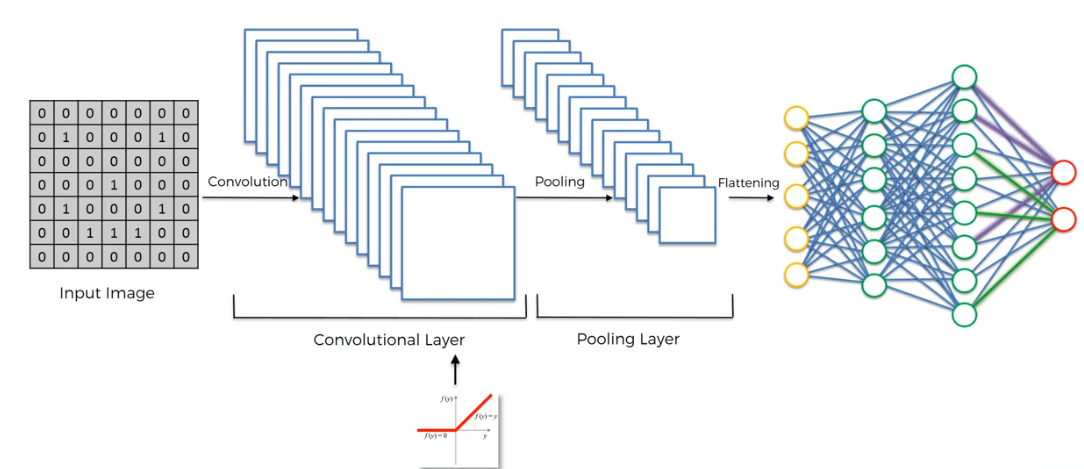
\includegraphics[height=0.25\textheight]  {CNN}}
\end{figure}

\subsubsection*{Convolutional layer.}
The input to the this layer is an image, which a computer views in terms of numbers of a matrix format as shown in the figure above.\\

In a Convolutional Neural Network the linear function that is used is called a convolutional layer. Each node
in the hidden layer extracts different features by using image processing feature detectors. For example, in
the first layer, the first node may extract the horizontal edges of an image, the second node may extract
vertical edges and etc. These features are extracted using a kernel. The figure below shows an example of how
strided convolutions work on an image. The bottom is the original image and the top is the output of the
convolutions. It is also worth noting that the output of the convolutions reduce the dimension of the original
image.\\

\begin{figure}[h]
	\centerline{\small 
		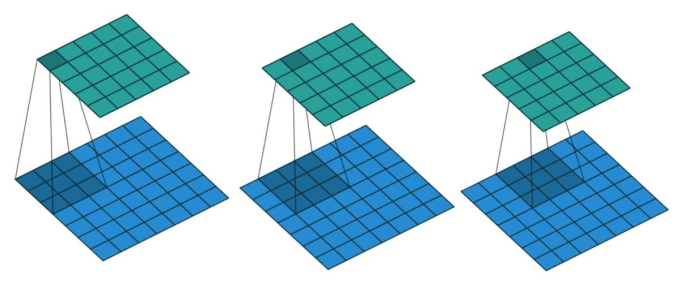
\includegraphics[height=0.25\textheight]  {f1}}
\end{figure}

\subsubsection*{ReLU layer.}
ReLU stands for Rectified Linear Units. The purpose of this layer is to introduce non-linearity in the system.
Until convolutional layer, the system has been making calculations linearly. In the past, sigmoid and tanh
functions were used to introduce non-linearity [80]. According to [79], ReLU layer applies max(0,x) to all the
activations formed by the convolutional layer. In naïve terms, the purpose of ReLU is to replace negative
activations by 0.\\


\subsubsection*{Pooling layer.}
The pooling layer happens tends to be computed after the convolutional layer. The reason why pooling is
done is to further reduce the dimensions of the convolutional layer and just extract out the features to make
the model more robust. There are two types of pooling done: max pooling and average pooling. Max pooling
extracts out the highest pixel value out of a feature while average pooling calculates the average pixel value
that has to be extracted. The figure below shows how the max and average pooling operation works.\\

\begin{figure}[h]
	\centerline{\small 
		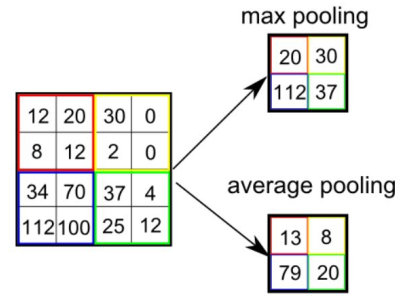
\includegraphics[height=0.25\textheight]  {f2}}
\end{figure}



\subsubsection*{Fully connected layer.}
The Fully Connected layer consists of the weights and biases along with the neurons and is used to connect the neurons between two different layers. These layers are usually placed before the output layer and form the last few layers of a CNN Architecture.

In this, the input image from the previous layers are flattened and fed to the Fully connected layer. The flattened vector then undergoes few more FC layers where the mathematical functions operations usually take place. In this stage, the classification process begins to take place.\\


\section{Convolutional Neural Networks (CNN) in Agriculture and its applications.}
For this research, we mainly focused on the application of Convolutional Neural Networks (CNN) in the Agricultural field.\\

\subsection{How CNN works.}
Recently, numerous types of deep learning architecture has been proposed for plant
disease classification. The most prominent technique is the convolutional neural network
(CNN). A convolutional neural network is a supervised deep learning model inspired by
the biological nervous system and vision system with significant performance compared
to other models. As compared to Artificial Neural Network (ANN), CNN requires few
neurons and multilayer convolution layers to learn the features, but it required an extensive
dataset for training [54,55].\\

In machine learning, CNN constitutes a class of deep, feed-
forward ANN that has been applied successfully to computer
vision applications [44,45].
In contrast to ANN, whose training requirements in terms of
time are impractical in some large-scale problems, CNN can learn
complex problems particularly fast because of weight sharing and
more complex models used, which allow massive parallelization [46]. Convolutional neural networks can
increase their probability of correct classifications, provided
there are adequately large data sets (i.e. hundreds up to thousands
of measurements, depending on the complexity of the problem
under study) available for describing the problem. They consist
of various convolutional, pooling and/or fully connected layers
[47]. The convolutional layers act as feature
extractors from the input images whose dimensionality is then
reduced by the pooling layers, while the fully connected layers
act as classifiers. Usually, at the last layer, the fully connected
layers exploit the high-level features learned, in order to classify
input images into predefined classes [48].
The highly hierarchical structure and large learning capacity of
CNN models allow them to perform classification and predictions
particularly well, being flexible and adaptable in a wide variety of
complex challenges [49].
Convolutional neural networks can receive any form of data as
input, such as audio, video, images, speech and natural language
[50,51,52,53], and have been applied suc-
cessfully by numerous organizations in various domains, such as
the web (i.e. personalization systems, online chat robots), health
(i.e. identification of diseases from MRI scans), disaster manage-
ment (i.e. identifications of disasters by remote-sensing images),
post services (i.e. automatic reading of addresses), car industry
(i.e. autonomous self-driving cars), etc.

\newpage
\subsection{Its application in agriculture.}
\begin{figure}[h]
	\centerline{\small 
		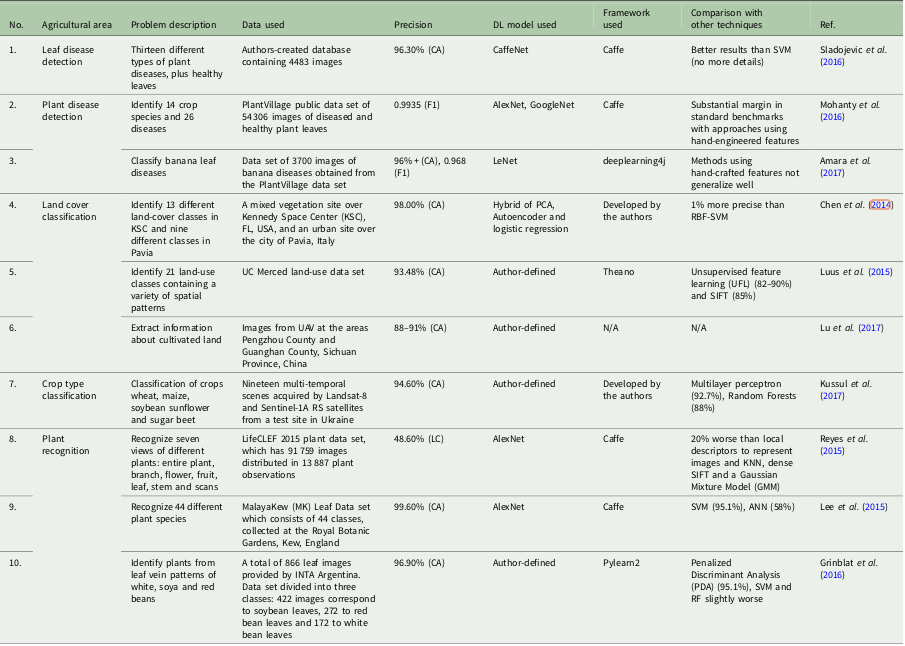
\includegraphics[height=0.5\textheight]  {agric}}
\end{figure}


\textbf{There are many methods to detect plant leaf diseases and various researchers had suggested various techniques for detecting irish potato leaf diseases in their work. In this section, a summary of those approaches is presented as below;}\\


In the last few decades, many researchers worked on multiple crops, including potatoes; their focus was not on the single potato crop diseases [25–27]. The models were
trained on specific region dataset (PlantVillage [28]), which was developed in the USA and
Switzerland. The diseases of potato vary from other regions due to the difference in leaf
shapes, varieties and environmental factors [29]. Geetharamani and Pandian [25] proposed
a deep CNN model to differentiate between healthy and unhealthy leaves of multiple
crops. The model was trained using the PlantVillage dataset with 38 different types of
crops with disease leaf images, healthy leaf images and background images. The focus
of the model was not on single potato crop diseases. The model is also trained in specific
region dataset USA and Switzerland, which failed to detect the Pakistani region potato
leaf diseases. Kamal et al. [26] developed plant leaf disease identification models named
Modified MobileNet and Reduced MobileNet using depthwise separable convolution
instead of convolution layer by modifying the MobileNet [30]. The proposed model was
trained on multiple crops of the PlantVillage dataset, where the plant leaf images were
collected from a specific region of the world. Khamparia et al. in [27], proposed a hybrid
approach to detect crop leaf disease using the combination of CNN and autoencoders. The model was trained on the PlantVillage dataset for multiple crop diseases and specific region
diseases. In [31], Liang et al. proposed a plant disease diagnosis and severity estimation
network based on a residual structure and shuffle units of ResNet50 architecture [56].
The PlantVillage dataset was also used to detect the multiple crop diseases of a specific
region. Ferentinos [57] investigated AlexNet [57], Overfeat [58], AlexNetOWTBn [59],
VGG [60] and GoogLeNet [61] deep learning-based architectures in order to identify the
normal or abnormal plants from plant leaf images. The researchers performed the transfer
learning approach using the PlantVillage dataset to detect the specific region’s multiple
crops diseases.
Many researchers worked on potato crops diseases but also trained the models on a
specific dataset PlanVillage. Khalifa et al. [62] proposed a CNN model to detect early blight
and late blight diseases along with a healthy class. The researchers trained their model on
the PlantVillage dataset, which is for specific regions’ crops only. Rozaqi and Sunyoto [63]
proposed a CNN model to detect the early blight, late blight disease of potato, and a
healthy class. They trained the model on the PlantVillage dataset to detect the diseases of a
specific region. Sanjeev et al. [64] proposed a Feed-Forward Neural Network (FFNN) to
detect early blight, late blight diseases along with healthy leaves. The proposed method
was trained and tested on the PlantVillage dataset. Barman et al. [65] proposed a self-build
CNN (SBCNN) model to detect the early blight, late blight potato leaf diseases, and healthy
class. The PlantVillage dataset was also used to train the model, which is for a specific
region. They did not validate their model on unseen test data. Tiwari et al. [66] used a
pre-trained model VGG19 to extract the features and used multiple classifiers KNN, SVM
and neural network for classification. The model also trained on the PlantVillage dataset to
detect the early blight and late blight disease of potato leaves. They did not test their model
on unseen data. Lee et al. [67] developed a CNN model to detect the early blight, late blight
diseases, and healthy leaves of potato. The researchers also used the PlantVillage dataset
belonging to a specific region. The model was not tested on unseen data. Islam et al. [68]
proposed a segment-based and multi-SVM-based model to detect potato diseases, such as
early blight, late blight and healthy leaves. Their method also used the PlantVillage dataset
and also needs to be improved in terms of accuracy.\\

\section{Convolutional Neural Networks (CNN) in other fields.}
In this section, we also looked at the applications of CNN in other fields of study other than Agriculture.\\

\subsection{Anomaly Detection.}
A CNN with 1-D convolutions was used on time series in the frequency domain (spectral residual) by an unsupervised model to detect anomalies in the time domain.[81] 

\subsection{Drug discovery.}
CNNs have been used in drug discovery. Predicting the interaction between molecules and biological proteins can identify potential treatments. In 2015, Atomwise introduced AtomNet, the first deep learning neural network for structure-based rational drug design.[82] The system trains directly on 3-dimensional representations of chemical interactions.\\

\subsection{Video analysis.}
Compared to image data domains, there is relatively little work on applying CNNs to video classification. Video is more complex than images since it has another (temporal) dimension. However, some extensions of CNNs into the video domain have been explored. One approach is to treat space and time as equivalent dimensions of the input and perform convolutions in both time and space.[83][84]\\

\subsection{Time series forecasting.}
Recurrent neural networks are generally considered the best neural network architectures for time series forecasting (and sequence modeling in general), but recent studies show that convolutional networks can perform comparably or even better.[85][86] Dilated convolutions[87] might enable one-dimensional convolutional neural networks to effectively learn time series dependences.[88] Convolutions can be implemented more efficiently than RNN-based solutions, and they do not suffer from vanishing (or exploding) gradients.[89] Convolutional networks can provide an improved forecasting performance when there are multiple similar time series to learn from.[90] CNNs can also be applied to further tasks in time series analysis (e.g., time series classification or quantile forecasting).

\subsection{Natural language processing.}
CNNs have also been explored for natural language processing. CNN models are effective for various NLP problems and achieved excellent results in semantic parsing,[91] search query retrieval,[92] sentence modeling,[93] classification,[94] prediction[95] and other traditional NLP tasks.[96] Compared to traditional language processing methods such as recurrent neural networks, CNNs can represent different contextual realities of language that do not rely on a series-sequence assumption, while RNNs are better suitable when classical time serie modeling is required.\\

\subsection{Health risk assessment and biomarkers of aging discovery}
CNNs can be naturally tailored to analyze a sufficiently large collection of time series data representing one-week-long human physical activity streams augmented by the rich clinical data (including the death register, as provided by, e.g., the NHANES study). A simple CNN was combined with Cox-Gompertz proportional hazards model and used to produce a proof-of-concept example of digital biomarkers of aging in the form of all-causes-mortality predictor.[97] 


\section{Existing methods used for Irish potato leaf disease detection.}
\begin{itemize}
	\item Manual observation using naked eyes.\\
	\item Hiring experts to manually detect the leaf diseases.\\
	
	
\end{itemize}

\section{Data sources.}
In this section, we used two datasets namely the Plant Village dataset and Potato Leaf Disease dataset to understand how the model works and performs on different sets of data.\\
To test our machine learning model, we used real Irish potato leaf images collected the gardens using our phone cameras.\\

\subsection{Plant Village Dataset description.}
In this study, Plant Village dataset [69] from Kaggle, a Data science website was used to design, build and train the machine model on known data.\\
The PlantVillage dataset was developed by Penn State University (US) and EPFL (Switzerland), which is a non-profit project. The
database consists of JPG colour images with 256 × 256 dimensions. It has 38 classes of diseased and healthy leaves of 14 plants. The focus of this research was on the Irish potato crop.
Therefore, 1000 leaves for late blight, 1000 leaves for early blight, and 152 images of healthy
leaves were selected for the experimental purposes, as shown below;\\
\begin{figure}[h]
	\centerline{\small 
		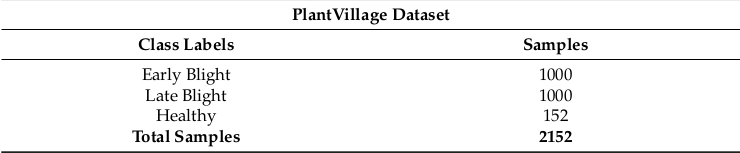
\includegraphics[height=0.1\textheight]  {l3}}
\end{figure}


\subsection{Potato Leaf Disease Dataset description.}
In the literature above, only the PlantVillage dataset has been used to develop the models
because only the PlantVillage dataset is publicly available for potato leaf diseases. All the
researchers used the PlantVillage dataset in their research, but there are many research
gaps found in the literature. The PlantVillage dataset has been developed from the specific
region under particular geography and environmental factors. There is variation in potato
diseases of different parts of the world due to variation in various factors such as shape,
varieties and environmental factors. Therefore, the existing systems have a high false
rate to recognize Irish potato disease detection in the leaf images.The PlantVillage dataset also has fewer images and an imbalanced
class distribution.\\

Therefore this dataset overcomes the errors of the Plant village dataset which include class imbalances, images with different sizes etc as discussed above.\\

The Potato Leaf Dataset (PLD) was developed from Pakistan’s Central
Punjab region by Directorate of Agriculture, Crop Reporting services, 2018 and Ministry of National food security and Research, 2019.\\

Unlike the Plant village dataset which consisted of many plant leaf images with their names grouped into their respective folders, this dataset (Potato Disease Leaf dataset) \textbf{only} had Irish potato leaf images. This dataset therefore overcomes some of the anomalies of the Plant village dataset which include class imbalances, images with different sizes, fewer images etc as discussed above.\\

This dataset consisted of 1628, 1414 and 1020 potato
leaf images for early blight, late blight and healthy classes, respectively as shown below.\\


\begin{figure}[h]
	\centerline{\small 
		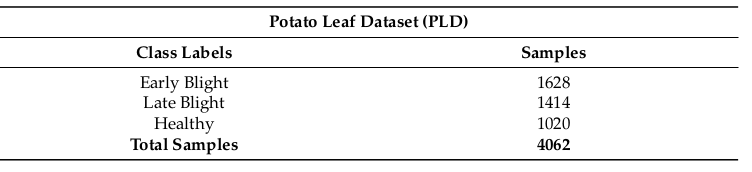
\includegraphics[height=0.11\textheight]  {hjk}}
\end{figure}





\newpage
\chapter{Research Methodology.}
\section{Introduction.}
In this part, we discuss methods and techniques we used to carryout our research.\\


\section{Research Design.}
The research design discusses various methods we used to accomplish the various activities we carried out.\\


\subsection{Studying or reviewing the existing literature.}
Using this research method, we collected information from already existing related research. Information was gathered from online sources such as the internet,journals, reports and also articles.\\

Many problems exist in the literature for the Plant Village dataset using deep learning approaches,
including incorrect identification of potato leaf diseases, variation in potato diseases, varieties and
environmental factors. The existing systems have a high false rate to recognize potato diseases in the
different regions of the world. The existing potato leaves disease datasets contain inadequate training
samples with imbalanced class samples. Another problem is that the current methods have a low con-
vergence speed due to the vast number of trainable parameters, and accuracy needs to be improved.
The last problem in the literature is the non-availability of the potato leaf segmentation technique.\\

With the help of the internet, journals, reports and also articles, we were able to study the existing systems with their loop holes that could be filled with our propose system.\\ 

\subsection{Interviews.}
This was a one to one discussion between the expected system users and the project team. With this
method the interviewer gets first-hand intelligence. The technique is also qualitative in nature and
helpful in validating the already gathered intel. On contrary there is a possibility of the interviewee
giving false intel when it comes to matters that involve emotions. The interviews were carried out
with some commercial Farmers nearby were team members met with growers of irish potatoes.\\

Information sought included;
\begin{itemize}
	\item Strengths and weaknesses of the current existing system or methods of disease detection and classification.
	
	\item Opinions on the proposed system for disease detection and classification.
\end{itemize}

This helped us to get a clear understanding of the current methods that farmers use to detect and classify leaf diseases. We were also able
to validate the information that was already gathered from other farmers.
On contrary there is a possibility of the interviewee giving false Intel when it comes to matters that
involve emotions.\\


Why we used interviews;

\begin{itemize}
	\item With this technique respondents are able to describe what is more important to them.\\
	\item There is a possibility of asking questions that are usually off the script.\\
	\item Quick responses from interviewees which reduces on the time of requirements collection.
\end{itemize}



\subsection{Data collection.}
The data collection process in this project was done using a number of data collection techniques
both qualitative and quantitative methods. The quantitative methods helped in evaluating the impact
of the current existing methods for disease detection and classification.\\

Learning farmers’ opinions
on a possibility of using our proposed system was a major drive to use qualitative
methods.
The data collection process in this project was done through interviews with the various
farmers of the system for example the farmers to identify the User Core Requirements.
Document reviews were also done in the process of data collection.\\

Datasets of leaf images were also downloaded from the internet for training our proposed model.\\ 

\subsection{Observation.}
With random visits we had to nearby Irish potato gardens, we saw some of the farmers use their naked eyes to carryout diagnosis to manually detect and classify leaf diseases and also determine if leaves are also healthy.\\

\section{Research Strategy.}
The research strategy discusses various tools we used to accomplish the various activities we carried out.\\

\subsection{Data collection.}
Two datasets were downloaded from the internet and also fresh leaf images were collected from nearby gardens.\\

Tools used;
\begin{itemize}
	\item Mozilla firefox web browser.
	\item Smartphone camera.
\end{itemize}

\subsection{Data preprocessing and cleansing.} 
This was through the following steps;

\begin{itemize}
	\item We Set constant values of batch sizes of 32, image size of 256 by 256, and channel size of 3 which
	was the RGB value importing them to the tensorflow dataset object.\\
	\item We prepared our data through allocating part of the training data, validation data, test data to
	80\%, 10\% and 10\% respectively through train-test split for each dataset.\\
	\item We applied Cache, Shuffle, and Prefetching to the Datasets.\\
	
	For caching, images were read from the disk for the next iteration when an image was needed,
	it kept that image in memory. hence improving the performance of the pipeline.\\
	
	For prefetch, if CPU and GPU were used, if GPU was busy training, prefetch would load the
	next set of batch from the disk and would improve the performance.\\
\end{itemize}

Tools used;
\begin{itemize}
	\item numpy library.
	\item pandas library.
	\item Scikit-learn.
	\item Jupyter notebook.
	\item Google Colab.
\end{itemize}



\subsection{Model formulation and building.}
This was through applying data augmentation to the training data.\\

Different data augmentation techniques were applied to the training set using the Image Data
Generator method of Keras library in Python to overcome overfitting and enhance the dataset’s
diversity. The computational cost was reduced using the smaller pixel values and the same
range; for this purpose, it used scale transformation. Therefore, every pixel value was ranged
from 0 to 1 using the parameter value (1./255). Images were rotated to a specific angle using
the rotation transformation; therefore, 25 degrees was employed to rotate the images. Images can shift
randomly either towards the right or left by using the width shift range transformation; selected
a 0.1 value of the width shift parameter. Training images moved vertically using the height shift
range parameter with a 0.1 range value.\\

For data augmentation to reduce overfitting, we considered an example of an image in the train-
ing data, 4 new samples are created from it eg rotation, horizontal flip, contrast and zoom
transformations thereby generating new training samples hence using all the 5 images for train-
ing making the model robust for unseen data or new images.\\

Tools used;
\begin{itemize}
	\item Keras library.
	\item OpenCV.
	\item TensorfFlow.
	\item Matplotlib.
	\item Jupyter Notebook.
	\item Google Colab.
\end{itemize}


\subsection{Model testing.}
This was through Compiling the Model using parameters like adam Optimizer, SparseCategoricalCrossentropy
for losses, accuracy as a metric with epoch values of 50.\\
We also used 10\% of the dataset to train our proposed model.\\

Tools used;
\begin{itemize}
	\item Jupyter notebook.
	\item Google colab.
	\item Spyder IDE for Anaconda.
\end{itemize}

\newpage
\chapter{Data collection, model building and Training.}
\section{Introduction.}
We collected data through downloading two datasets namely the publicly known Plant Village dataset form Kaggle website and the Potato Disease Leaf Dataset from Plant disease research repository website all using Mozilla firefox web browser.\\

To test our model, we collected fresh leaf images of Irish potatoes from near by gardens using a smartphone camera with a high resolution to enhance high image quality.\\

\section{Dataset description.} 
\subsection{Plant Village dataset.}
This dataset which is publicly available on Kaggle website consisted of JPG colour images with 256 × 256 dimensions. It had 38 classes of diseased and healthy leaves
of 14 plants. The focus of the research was on the Irish potato crop.\\
Plant leaf images with their names were grouped into respective folders, so we had to delete all non Irish potato folders to  remain with the relevant crop which was Irish potatoes for this research study.\\

Therefore, 1000 leaves for
late blight, 1000 leaves for early blight and 150 images of healthy leaves were selected for
the experiment. Then the dataset was divided into 80\%, 10\% 10\% ratios for train, validation
and test sets. The training set consisted of 800 images of early blight, 125 images of healthy
leaves and 800 images of late blight class; for the validation set, 100, 100 and 14 images of
early blight, late blight and healthy, respectively. The test set contained 100, 100 and 13
images of early blight, late blight and healthy.\\

\begin{figure}[h]
	\centerline{\small 
		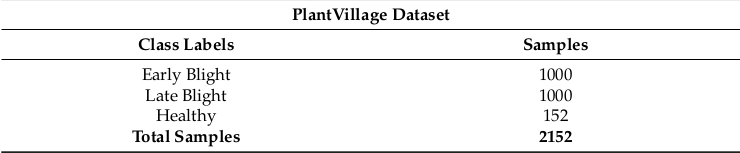
\includegraphics[height=0.1\textheight]  {l3}}
\end{figure}

\subsection{Potato Disease Leaf dataset.}
In the literature section 2.0, only the PlantVillage dataset has been used to develop the models
because only the PlantVillage dataset is publicly available for potato leaf diseases. All the
researchers used the PlantVillage dataset in their research, but there are many research
gaps found in the literature. The PlantVillage dataset has been developed from the specific
region under particular geography and environmental factors. There is variation in potato
diseases of different parts of the world due to variation in various factors such as shape,
varieties and environmental factors. Therefore, the existing systems have a high false
rate to recognize Irish potato disease detection in the leaf images.The PlantVillage dataset also has fewer images and an imbalanced
class distribution.\\


The Potato Leaf Dataset (PLD) was developed from Pakistan’s Central
Punjab region by Directorate of Agriculture, Crop Reporting services, 2018 and Ministry of National food security and Research, 2019.\\

Unlike the Plant village dataset which consisted of many plant leaf images with their names grouped into their respective folders, this dataset (Potato Disease Leaf dataset) \textbf{only} had Irish potato leaf images. This dataset therefore overcomes some of the anomalies of the Plant village dataset which include class imbalances, images with different sizes, fewer images etc as discussed above.\\

This dataset consisted of 1628, 1414 and 1020 potato
leaf images for early blight, late blight and healthy classes, respectively as shown below.\\

\begin{figure}[h]
	\centerline{\small 
		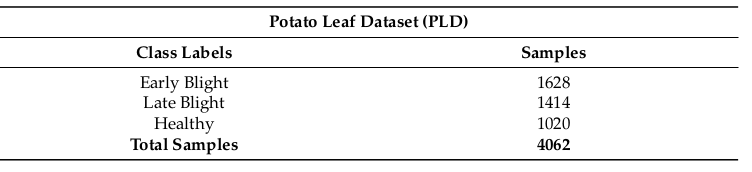
\includegraphics[height=0.11\textheight]  {hjk}}
\end{figure}

\section{Technology decisions.}
\subsection{Overview.}
In this section, we discuss details about the technologies that we used for this project. Although there were many
tools that existed out there in the market, we found out that these tools outlined performed well for the
problem that needed to be solved.\\

\subsection{Python.}
Python is a high level interpreted language used for general purpose programming. It is widely used for
scientific computing and can be used for a wide variety of general tasks from data mining to software
development. Python was the main language used for this project.\\

\subsection{Anaconda.}
Anaconda is a popular data science platform where you can create data science projects and machine
learning.[70]. Libraries such as NumPy, Pandas, Matplotlib, Tensorflow and etc come with Anaconda and
IDE’s such as Jupyter Notebook, Spyder and etc.\\

\subsection{Numpy.}
Numpy is a library in Python that allows for efficient numerical computing in Python. This library is highly
optimized to do mathematical tasks. In the project workflow Numpy is heavily used in data pre-processing
and preparation One of the main features about Numpy is it’s highly efficient n-dimensional array (ndarray).
Compared to a list in Python a Numpy array can be n-dimensions and has more features associated with the
ndarray. Numpy can also perform more efficient mathematical operations compared to the math library in
Python.\\

\subsection{Pandas.}
Pandas is also a library in Python, like numpy is also used for data pre-processing and preparation. One
of the main features about pandas is the DataFrame and Series data structure. These data structures are
optimized and contain fancy indexing that allow a variety of features such as reshaping, slicing, merging,
joining and etc to be available.
Pandas and Numpy are extremely powerful when used together for manipulating data.\\

\subsection{Matplotlib.}
Matplotlib is a Python plotting library that allows programmers to create a wide variety of graphs and
visualizations with ease of use. The great feature about Matplotlib is that it integrates very well with
Jupyter Notebook and creating visualizations is simplified. Matplotlib also works very well with pandas and
numpy.\\

\subsection{OpenCV.}
OpenCV (Open Source Computer Vision) is a well established computer vision library which is written in
C/C++ and has been abstracted to interface with C++, Python and Java. This is a powerful tool when
working with images and has a myriad of tools regarding image data manipulation, feature extraction and
etc.\\

\subsection{Tensorflow.}
Tensorflow is an open source deep learning library by Google. It was originally developed by Google’s
engineers who were working on Google Brain and has been used for research on machine learning and deep
learning. Tensorflow at it’s core is about computations of multidimensional arrays called tensors but what
makes Tensorflow great is its ability to be flexible to deploy computations on different devices such as CPU’s
and GPU’s [71].\\

\subsection{Keras.}
Keras is also a Deep Learning Framework that abstracts much of the code in the other Frameworks like
Tensorflow and Theano. Compared to the other frameworks Keras is more minimalist[72].\\

\subsection{Jupyter Notebook IDE.}
The Anaconda distribution comes with a variety of software that includes Jupyter Notebooks for scientific
computing. Jupyter Notebooks[73] is an open source software IDE that allows developers to create and share
documents that contain live code and more.\\

\subsection{Google Colab.}
Google Colab is a Deep Learning Platform in the Cloud[74]. Google Colab allows developers to run heavy tasks on
the cloud such as training the deep learning model or heavy preprocessing tasks. The CPU’s and GPU’s
available on Google Colab are fully configured to work on different Frameworks such as Tensorflow. One of the
main benefits to Google Colab is that it is quite powerful and easy to use with easy to follow documentation.\\


\section{Experimental tests.}
We performed experimental test methods to better understand how the machine learning model works on both datasets ie the publicly known Plant village dataset and Potato Disease leaf dataset.\\

Model experiments were conducted while in Google Colab on the machine learning model and the results focused on the following;
\begin{itemize}
	\item Differentiating the potato leaf images into early blight, late blight, or healthy.\\
	\item The evaluation of our model’s performance on the Potato disease leaf dataset using data augmentation and without data augmentation techniques on the training set.\\
	\item The evaluation of our model’s performance on the publicly
	available dataset ie PlantVillage by applying data augmentation and without data augmentation techniques.
	\item We measured the performance of the proposed model on the cross dataset.\\
	\item To evaluate the results of potato leaf disease detection with existing studies using
	deep learning.\\
\end{itemize}


Since the Plant Village dataset had many anomalies, data augmentation techniques were applied to four sets to the Potato Leaf Disease dataset shown below;\\

\begin{figure}[h]
	\centerline{\small 
		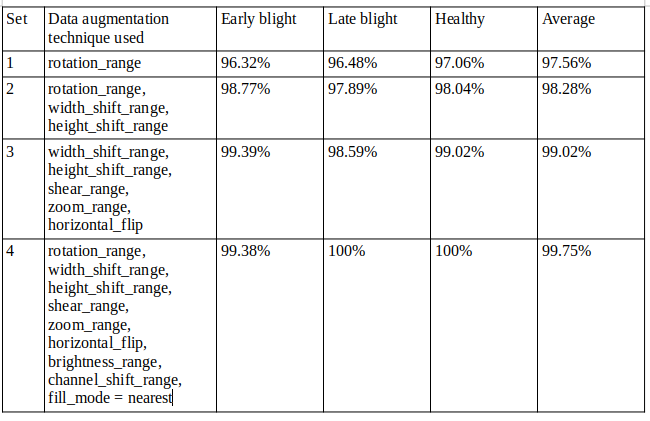
\includegraphics[height=0.3\textheight]  {diag}}
\end{figure}

Therefore, as we increased the training samples using more data augmentation techniques, the overall accuracy increased. The fourth set archived the highest accuracy because we increased the training samples using the seven data augmentation techniques.\\  





\newpage
\section{Steps taken to build the machine learning model.}
Here we took the following steps to come up with our machine learning model.\\

\subsection{Data preparation.}

\begin{itemize}
	\item Setting constant values of batch sizes of 32, image size of 256 by 256, and channel size of 3 which is the RGB value importing them to the tensorflow dataset object.\\
	\item Since the PlantVillage dataset contained 3 classes ie Early blight, Late blight and the Healthy class, We prepared our data through allocating part of the training data, validation data, test data to 80\%, 10\% and 10\% respectively through train-test split.\\ 
	\item Cache, Shuffle, and Prefetching the Dataset. 
	
	For caching, an image is read from the disk for the next iteration when an image is needed, it will keep that image in memory. hence improving the performance of the pipeline.\\
	
	For prefetch, if CPU and GPU are used, if GPU is busy training, prefetch will load the next set of batch from the disk and will improve the performance.\\
	
	
\end{itemize}


\subsection{Model formulation/Model building.}
\begin{itemize}
	\item This was through data pre-processing ie 
	Creating a Layer for Resizing and Normalization.\\
	
	Before feeding our images to the network, we resized it to the desired size. Moreover, to improve model performance, we normalized the image pixel value (keeping them in range 0 and 1 by dividing by 256). This happened while training as well as inference. Hence we added that as a layer in our Sequential Model.\\
	
	we needed to resize (256,256) image to again (256,256) since this was useful when we were done with the training and started using the model for predictions. At that time, some one could have supplied an image that is not (256,256) and this layer would resize it.\\
	
	\item Applying Data Augmentation to the training data.\\
	Data Augmentation was needed when we had less data, this boosted the accuracy of our model by augmenting the data.\\
	
	For data augmentation to reduce overfitting, we considered an example of an image in the training data, 4 new samples are created from it eg rotation, horizontal flip, contrast and zoom transformations thereby generating new training samples hence using all the 5 images for training making the model robust for unseen data or new images.\\
	
	Different data augmentation techniques were applied to the training set using the
	Image Data Generator method of Keras library in Python to overcome overfitting and
	enhance the dataset’s diversity. The computational cost was reduced using the smaller
	pixel values and the same range; for this purpose, it used scale transformation. Therefore,
	every pixel value was ranged from 0 to 1 using the parameter value (1./255). Images were
	rotated to a specific angle using the rotation transformation; therefore, 25 ◦ was employed
	to rotate the images. Images can shift randomly either towards the right or left by using the
	width shift range transformation; selected a 0.1 value of the width shift parameter. Training images moved vertically using the height shift range parameter with a 0.1 range value.\\
	
	\item Coming up with the CNN architecture with layers like initial layers for resizing, normalization and Data Augmentation.\\
	
	We used a CNN coupled with a Softmax activation in the output layer.\\ 
	\begin{figure}[h]
		\centerline{\small 
			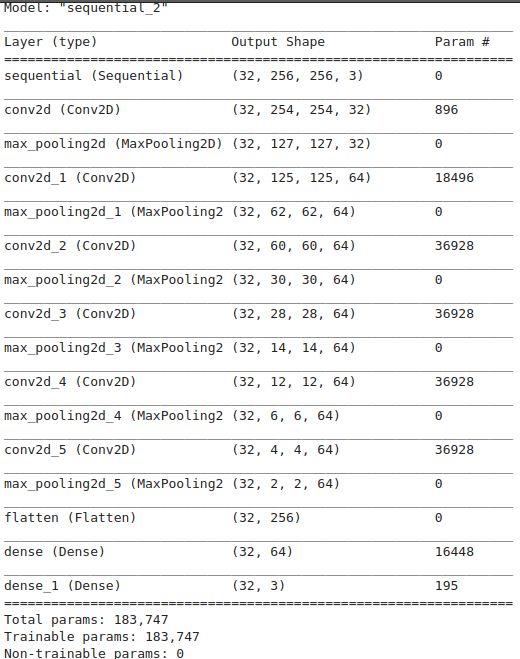
\includegraphics[height=0.5\textheight]  {x12}}
	\end{figure}
	
\end{itemize}


\newpage
\subsection{Model implementation.}
\begin{itemize}
	\item This was through Compiling the Model using adam Optimizer, SparseCategoricalCrossentropy for losses, accuracy as a metric with epoch values of 50.\\
	Sample results below after running the model with accuracy of 100\% and value loss of 0.0064.\\
	\begin{figure}[h]
		\centerline{\small 
			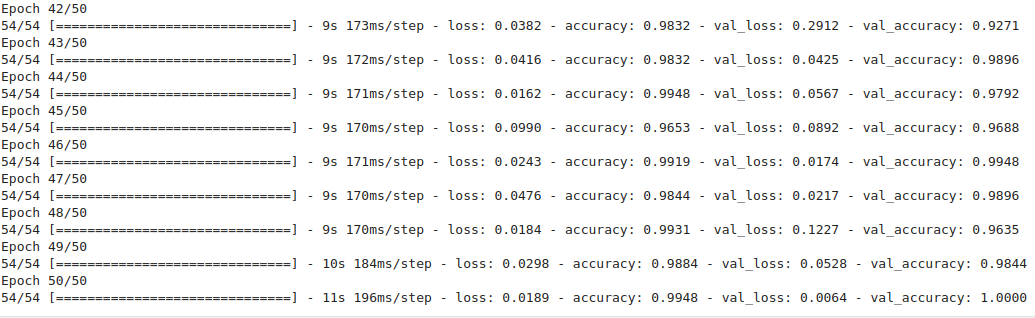
\includegraphics[height=0.2\textheight]  {vt}}
	\end{figure}
	
	
\end{itemize}




\subsection{Evaluation metrics.}
We evaluated our model by plotting Training and Validation accuracy, loss curves as below which showed the model performance with curves for easy visualization.\\
\begin{itemize}
	\item For the Training and Validation accuracy curves on the left, our model performed very well on training data and validation data allocated to it as it learned more accurately to the extent of reaching above to value of one.\\
	\item For the Training and Validation loss curves on the right, as our model learned with more data accurately, errors were few and curves declined down to the right.\\  
\end{itemize}
\begin{figure}[h]
	\centerline{\small 
		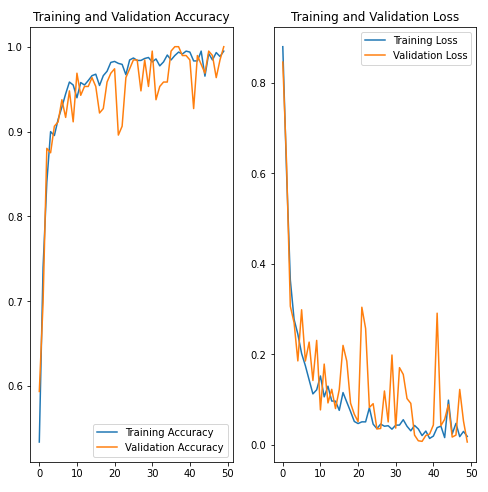
\includegraphics[height=0.35\textheight]  {bn}}
\end{figure}

\newpage
\section{Results/Performance.}

\subsection{Evaluation Measures.}
\subsubsection*{Classification accuracy.}
Classification accuracy is calculated by the number of correct predictions divided by
the total number of accurate predictions.\\

Accuracy = $\frac{Number of Correct Predictions}{Total Number of Predictions}$



\subsubsection*{Recall.}
The recall is another critical metric, characterised as the division of input samples
from a class accurately anticipated by the model. The recall is calculated as:\\

Recall = $\frac{TP}{(TP + FN)}$

\subsubsection*{F1 Score.}
One well-known metric that combines precision and recall is called the F1-score, which
is defined as:\\

F1 score = $\frac{2 * Precision * Recall}{(Precision + Recall)}$

\subsubsection*{Precision.}
There are numerous cases in which classification accuracy is not a significant pointer
to measure the model’s performance. One of these scenarios is when class dissemination
is imbalanced. If you anticipate all samples as the top class, you will get a high accuracy
rate, which does not make sense (since the model is not learning anything, and it is fair
foreseeing everything as the best class. Subsequently, precision describes the inconsistency
you find when using the same instrument; you repeatedly measure the same part. Precision
is one of such measures, which is characterised as:\\

Precision = $\frac{TP}{(TP + FP)}$


\subsection{Discussion of the results.}

\subsection*{A: Plant Village dataset.}
Classification accuracies, precision, recall and F1-Score of our model on this dataset.\\

\begin{itemize}
	\item With data augmentation;\\
	Performance measures\hspace{3cm}Early blight\hspace{2cm}Late blight\hspace{2cm}Healthy\\
	\textbf{Accuracy}\hspace{6cm}99\%\hspace{2cm}95\%\hspace{4cm}92.31\%
	\textbf{Precision}\hspace{6cm}95\%\hspace{2.5cm}98\%\hspace{4cm}100\%
	\textbf{Recall}\hspace{6.5cm}99\%\hspace{2.5cm}95\%\hspace{4cm}92\%
	\textbf{F1 score}\hspace{6cm}97\%\hspace{2.5cm}96\%\hspace{4cm}96\%
	Average accuracy: 96.71\%
	
\end{itemize}



\begin{itemize}
	\item Without data augmentation;\\
	Performance measures\hspace{3cm}Early blight\hspace{2cm}Late blight\hspace{2cm}Healthy\\
	\textbf{Accuracy}\hspace{6cm}91\%\hspace{3cm}96\%\hspace{3cm}100\%
	\textbf{Precision}\hspace{6cm}97\%\hspace{3.5cm}91\%\hspace{3cm}93\%
	\textbf{Recall}\hspace{6.5cm}91\%\hspace{3.5cm}96\%\hspace{3cm}100\%
	\textbf{F1 score}\hspace{6cm}94\%\hspace{3.5cm}94\%\hspace{3cm}96\%
	Average accuracy: 93.90\%
	
\end{itemize}

(a) Accuracy graph of our model on PlantVillage dataset with data augmentation. (b) Accuracy graph of our model on PlantVillage dataset without data augmentation;\\

\begin{figure}[h]
	\centerline{\small 
		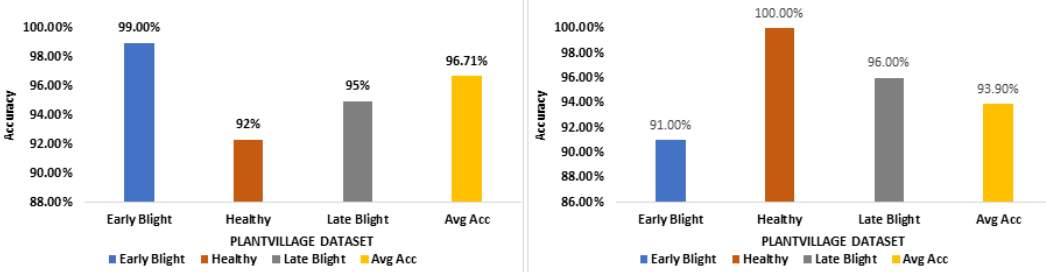
\includegraphics[height=0.17\textheight]  {v1}}
\end{figure}

\subsubsection*{Accuracy and Loss graph of model on dataset using data augmentation.}
The complete training and validation accuracies and losses of each epoch
were shown in the figure below. The results showed that the model achieved excellent
identification rates when the data augmentation techniques applied the training set of the
PlantVillage dataset, which indicated the model’s generalisation.\\

(a) Accuracy graph of our model on PlantVillage dataset using data augmentation. (b) Loss graph of our model on PlantVillage dataset using data augmentation;\\

\begin{figure}[h]
	\centerline{\small 
		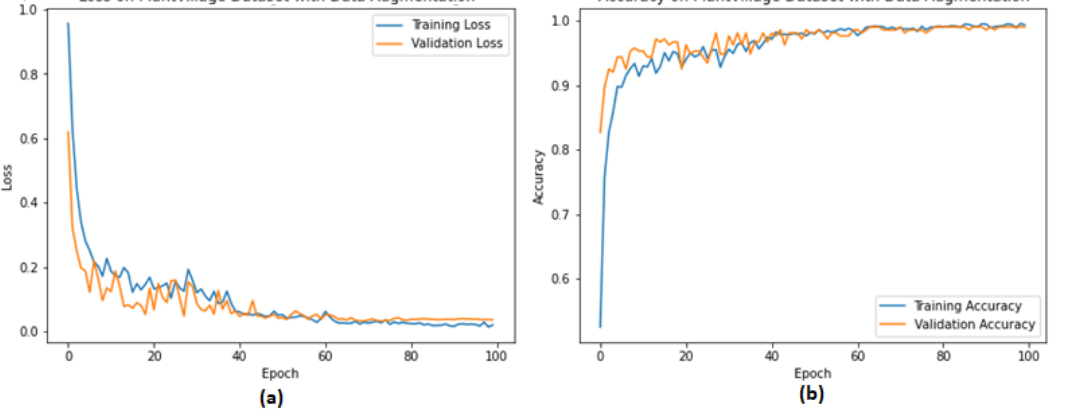
\includegraphics[height=0.17\textheight]  {v2}}
\end{figure}

\subsubsection*{Precision, Recall, F1 score.}
The model was further examined by calculating the test set’s precision, recall
and F1-score. It also observed that the model’s performance achieved
excellent results using the data augmentation techniques applied to the training set of the
PlantVillage dataset, as in the figure below. On the dataset, the model achieved 95\%, 100\% and 98\% precision on early blight, healthy and late blight,
respectively. It attained 99\%, 92\% and 95\% recall for early blight, healthy and late blight
classes and 97\%, 96\% and 96\% F1-scores on early blight, healthy and late blight. The results
presented an excellent performance on all the classes of the PlantVillage dataset using data
augmentation techniques.\\

(a) precision, recall and F1-Score on PlantVillage with data augmentation.
(b) precision, recall and F1-Score on PlantVillage without data augmentation;\\

\begin{figure}[h]
	\centerline{\small 
		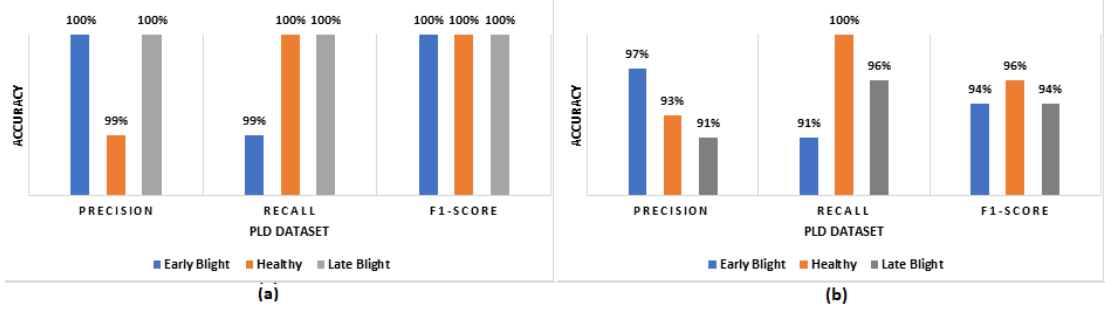
\includegraphics[height=0.17\textheight]  {v3}}
\end{figure}

\newpage
\subsubsection*{Confusion matrix.}
The model correctly identified 99 early blight diseased images out of 100 images, 12 healthy leaves
out of 13 leaves, and 95 early blight leaves out of 100 leaf images. The overall classification
accuracy of the model was 96.71\% on the PlantVillage dataset with
data augmentation techniques applied to the training set. The model’s mis-classification ratio was 3.29\% on all classes when data augmentation techniques were applied to
the training set on the PlantVillage dataset. The results confirmed that the model achieved excellent prediction accuracy using data augmentation techniques
applied to a training set of both the PLD and PlantVillage dataset.\\

(a) confusion matrix on PlantVillage with augmentation. (b) confusion matrix on PlantVillage without augmentation;\\
\begin{figure}[h]
	\centerline{\small 
		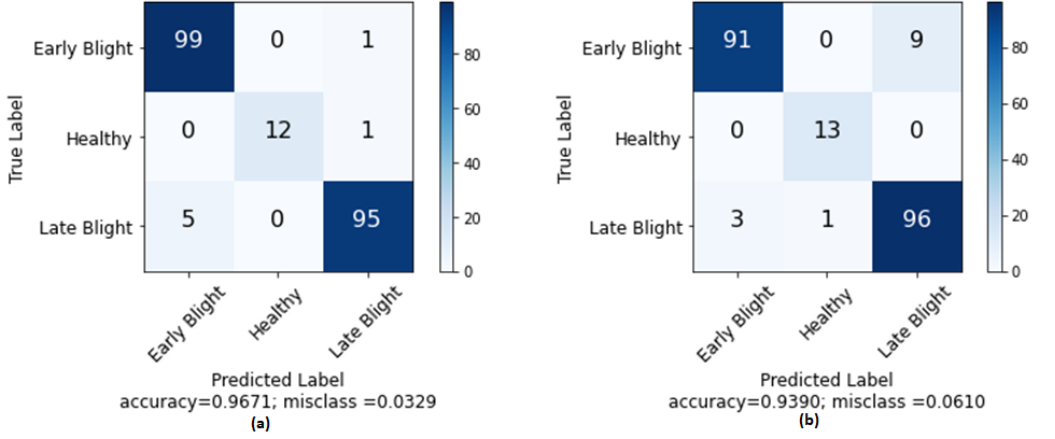
\includegraphics[height=0.17\textheight]  {v4}}
\end{figure}


\subsubsection*{ROC curve.}
ROC was also measured to confirm the proposed method’s performance on the PlantVillage dataset using data augmentation techniques, as presented in the figure below.
The light blue color indicates the early blight. The orange color denotes a healthy
class. The green color represents the late blight class, and the blue colour represents
the random guessing. The ROC curve graph showed that the early blight achieved 97\%, healthy achieved 96\%, and late blight achieved 97\% area under the curve, representing
good classification performance under the curve on the PlantVillage dataset using data
augmentation techniques applied to the training set of the model. All
the evaluation measures showed that the proposed method achieved a lower accuracy on
the PlantVillage dataset than the PLD dataset. The latter had more data for training the
proposed model and, therefore, possessing more accuracy than the PlantVillage dataset.\\

\newpage
The ROC curve, was used to assess the model’s
performance on the PlantVillage dataset without using data augmentation techniques, as
shown in Figure b. The light blue color indicates the early blight, and the orange colour
represents the healthy class. The green color denotes the late blight class, and the blue
color denotes random guessing. The ROC curve graph showed that the early blight had
94\%, healthy had 100\% and late blight had 94\% area under the curve.\\


(a) Model's ROC Curve on PlantVillage dataset with Augmentation. (b) Model's ROC Curve on PlantVillage dataset without augmentation;\\

\begin{figure}[h]
	\centerline{\small 
		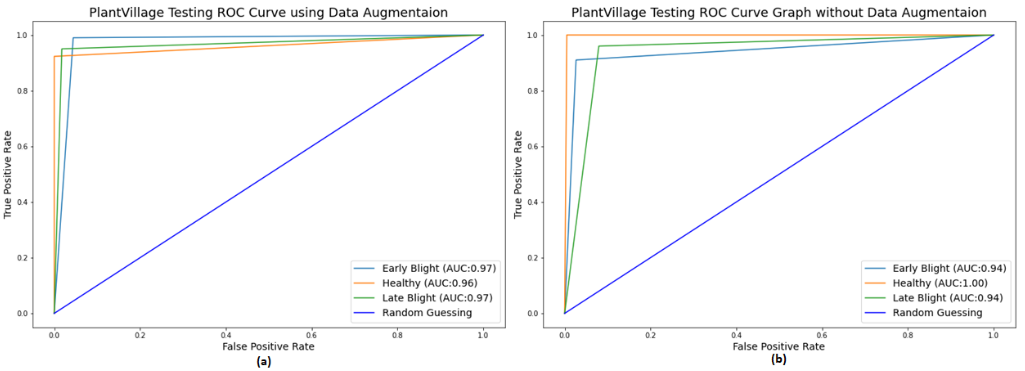
\includegraphics[height=0.17\textheight]  {v5}}
\end{figure}

\subsubsection*{Accuracy and Loss graph of model on dataset without data augmentation.}

The complete training and validation
accuracies and losses are shown in the figure below, depicting the model’s
overall performance on the dataset without data augmentation techniques
applied to the training set.\\

(a) Accuracy graph of model on PlantVillage dataset without data augmentation. (b) Loss
graph of model on PlantVillage dataset without data augmentation;\\

\begin{figure}[h]
	\centerline{\small 
		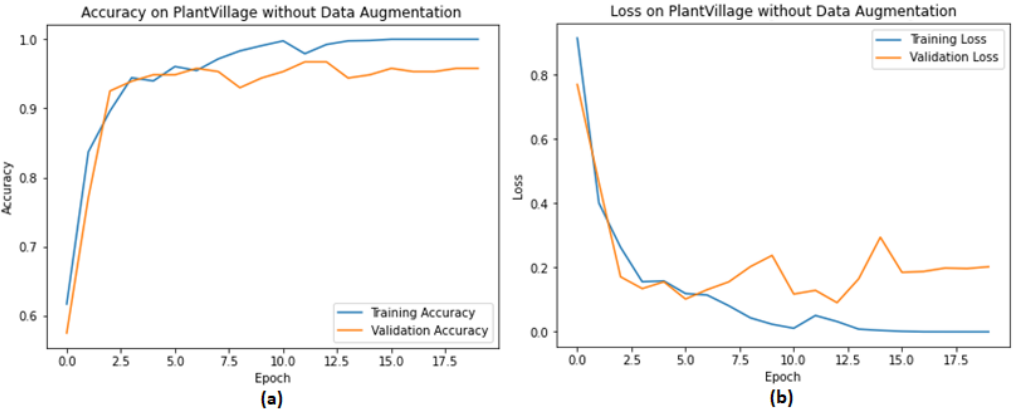
\includegraphics[height=0.17\textheight]  {v6}}
\end{figure}

\subsubsection*{Conclusion.}
All results depicted the model achieved less accurate performance when data augmentation techniques were not applied to the training set of the
PlanVillage dataset. The reason was that the model had less data to train. The
deep learning method needed a massive amount of data to train. Therefore, to enhance the
performance of the model, the dataset should be very large.\\


\newpage
\subsection*{B: Potato Leaf Disease dataset.}
Classification accuracies, precision, recall and F1-Score of our model on this dataset.\\

\begin{itemize}
	\item With data augmentation;\\
	Performance measures\hspace{3cm}Early blight\hspace{2cm}Late blight\hspace{2cm}Healthy\\
	\textbf{Accuracy}\hspace{6cm}99.38\%\hspace{3cm}100\%\hspace{2.5cm}100\%
	\textbf{Precision}\hspace{6cm}100\%\hspace{3.5cm}100\%\hspace{2.5cm}99\%
	\textbf{Recall}\hspace{6.5cm}99\%\hspace{3.5cm}100\%\hspace{2.5cm}100\%
	\textbf{F1 score}\hspace{6cm}100\%\hspace{3.5cm}99\%\hspace{2.5cm}100\%
	Average accuracy: 99.75\%
	
\end{itemize}


\begin{itemize}
	\item Without data augmentation;\\
	Performance measures\hspace{3cm}Early blight\hspace{2cm}Late blight\hspace{2cm}Healthy\\
	\textbf{Accuracy}\hspace{6cm}93.87\%\hspace{3cm}92.25\%\hspace{2cm}84.47\%
	\textbf{Precision}\hspace{6cm}87\%\hspace{3.5cm}90\%\hspace{3cm}94\%
	\textbf{Recall}\hspace{6.5cm}92\%\hspace{3.5cm}88\%\hspace{3cm}85\%
	\textbf{F1 score}\hspace{6cm}96\%\hspace{3.5cm}94\%\hspace{3cm}92\%
	Average accuracy: 91.15\%
	
\end{itemize}


The results above showed how the model achieved with the seven data augmentation techniques achieved in the 3.3.3 section: Experimental tests set 4 of the table.\\

Accuracy graph of model with data augmentation on the dataset;\\
\begin{figure}[h]
	\centerline{\small 
		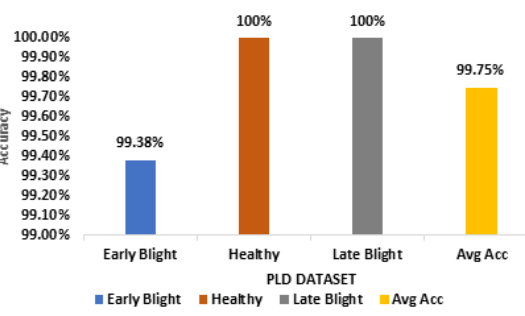
\includegraphics[height=0.2\textheight]  {p1}}
\end{figure}

Accuracy graph of the model without data augmentation on the dataset;\\
\begin{figure}[h]
	\centerline{\small 
		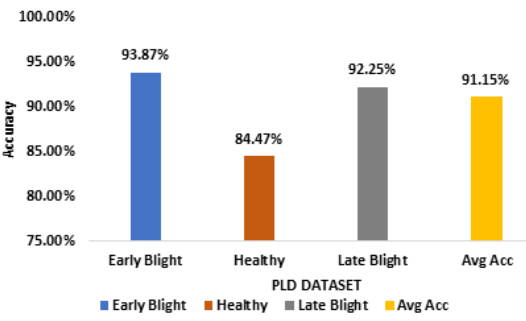
\includegraphics[height=0.2\textheight]  {p2}}
\end{figure}

\newpage
\subsubsection*{Accuracy and Loss curves on dataset with data augmentation.}

The
complete training, validation accuracy and losses in each epoch are depicted in the figures below,
showing the model’s overall performance on the dataset using
the data augmentation techniques applied to the training set. The results showed that the model achieved excellent identification rates on the dataset using the data
augmentation techniques applied to the training set.\\

Accuracy graph of our model on the dataset using data augmentation;\\
\begin{figure}[h]
	\centerline{\small 
		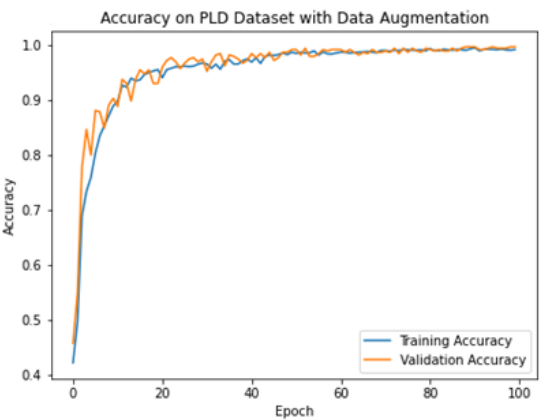
\includegraphics[height=0.25\textheight]  {p3}}
\end{figure}

Loss graph of our model on the dataset using data augmentation;\\
\begin{figure}[h]
	\centerline{\small 
		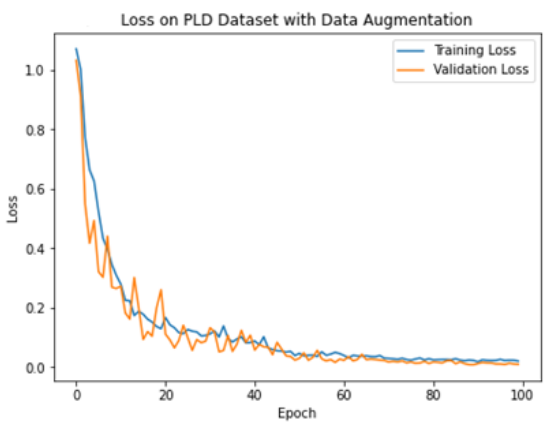
\includegraphics[height=0.25\textheight]  {p4}}
\end{figure}

\newpage
\subsubsection*{Precision, Recall and F1 score.}
The figures below demonstrated that the model achieved 100\%, 99\% 100\% precision scores on early blight, healthy and
late blight and attained 99\%, 100\% 100\% recall scores on early blight, healthy and late
blight. The model also achieved 99\%, 100\% 100\% F1-scores on early
blight, healthy and late blight using data augmentation techniques on the dataset.
The results showed excellent performance on all the classes of the  dataset.\\


precision, recall and F1-Score on the dataset with data augmentation;\\
\begin{figure}[h]
	\centerline{\small 
		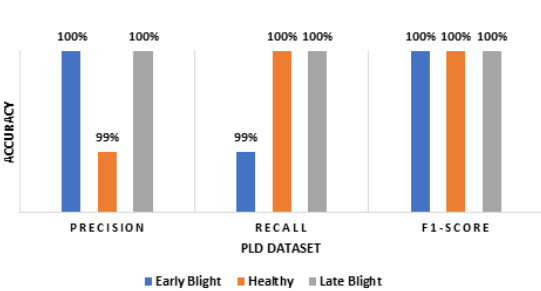
\includegraphics[height=0.25\textheight]  {p5}}
\end{figure}

precision, recall and F1-Score on the dataset without data augmentation;\\
\begin{figure}[h]
	\centerline{\small 
		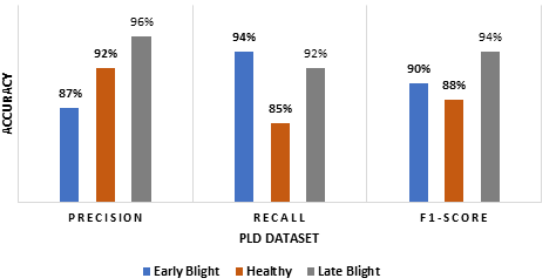
\includegraphics[height=0.25\textheight]  {p6}}
\end{figure}

\newpage
\subsubsection*{Confusion matrix.}
The confusion matrix is a valuable Machine Learning method that calculates the precision, recall, accuracy and AUC-ROC curve. A confusion matrix was utilized to
estimate the classification accuracy of a model visually. In the confusion matrix, correct
predictions were exhibited diagonally, and incorrect predictions were shown off-diagonally.
It represented the higher classification accuracy of the model of the corresponding class in a dark colour, and a lighter colour meant the misclassified samples. The results showed
that the model performed significantly when data augmentation
techniques were applied.\\


The confusion matrix of our model on the dataset with augmentation;\\
For Early blight class, there were 163 correct predictions with zero or no incorrect predictions at all.\\
For the Healthy class, there were 102 correct predictions with zero or no incorrect predictions at all.\\
For Late blight class, there were 142 correct predictions with zero or no incorrect predictions at all.\\
\textbf{This was an evaluation technique.}\\
\begin{figure}[h]
	\centerline{\small 
		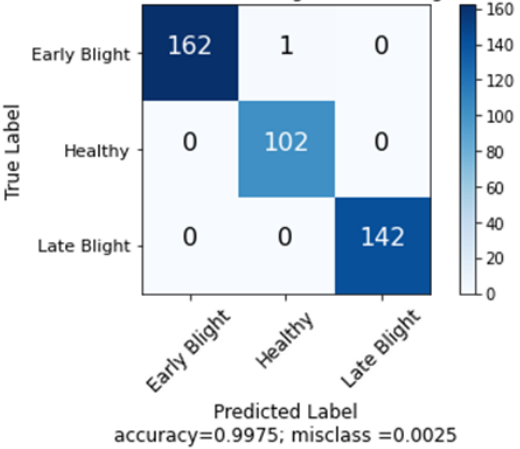
\includegraphics[height=0.25\textheight]  {p7}}
\end{figure}

The confusion matrix of our model on the dataset without augmentation;\\
For the Early blight class, there were 153 correct predictions with 10 incorrect predictions.\\
For the Healthy class, there were 87 correct predictions with 15 incorrect predictions.\\
For the Late blight class, there were 131 correct predictions with 11 incorrect predictions.\\
\begin{figure}[h]
	\centerline{\small 
		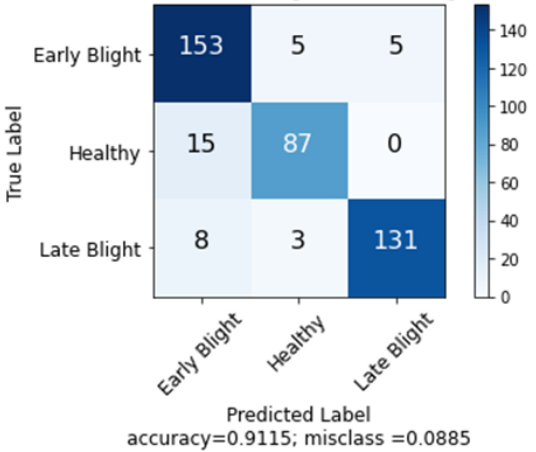
\includegraphics[height=0.25\textheight]  {p8}}
\end{figure}

\newpage
\subsubsection*{ROC curve.}
The model’s performance was measured using the ROC curve shown in the figures below. The light blue color indicates the early blight. The orange color represents
the healthy class. The green color represents the late blight class, and the blue color
shows the random guessing. All classes that showed a larger area (almost 100\%) under the curve present excellent classification performance of the model on the validation
and test set.\\

(a) ROC curve on the dataset with augmentation techniques. (b) ROC curve on the dataset without augmentation techniques;\\
\textbf{The graph on the left showed an excellent evaluation since all class curves headed to 1.}\\
\begin{figure}[h]
	\centerline{\small 
		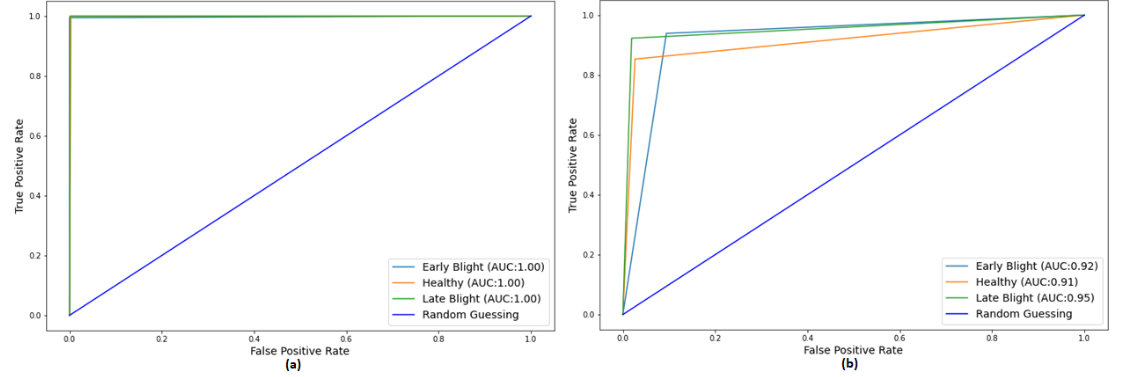
\includegraphics[height=0.2\textheight]  {p9}}
\end{figure}


\subsubsection*{Accuracy and Loss curves on dataset without data augmentation.}
The complete training and validation accuracy and losses in each epoch are shown in the figure below. The model achieved lower identification rates without using data augmentation techniques
compared to using data augmentation techniques applied to the training set. Therefore, for better classification accuracy, it should train on a large-scale dataset.
The model’s performance was further examined by calculating
the precision, recall and F1-score on each class’s validation set and testing set. The model did not achieve better results when data augmentation techniques were
not applied to the training set. The model achieved 87\%, 94\% and 90\% precision on early blight,
healthy and late blight, respectively, 92\%, 85\% and 88\% recall for early blight, healthy
and late blight, respectively, and it achieved 96\%, 92\% and 94\% F1-scores on early blight,
healthy and late blight. The results showed lower performance on all the classes than
when data augmentation was applied to the dataset training set. The reason for lower
performance was that the model was trained on a limited dataset.\\


(a) Accuracy graph of our model on the dataset without data augmentation. (b) Loss graph of our model on the dataset without data augmentation;\\
\begin{figure}[h]
	\centerline{\small 
		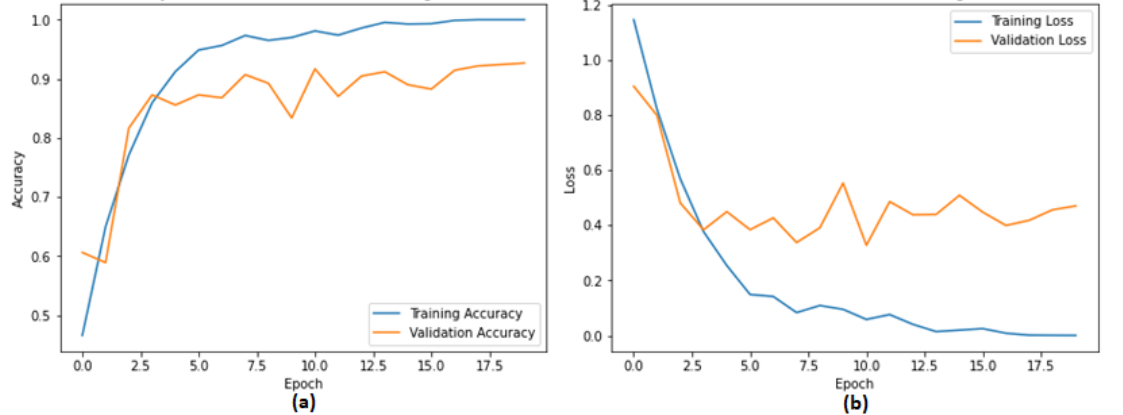
\includegraphics[height=0.20\textheight]  {p10}}
\end{figure}

\subsubsection*{Conclusion.}
All the evaluation measures demonstrated the model’s lower performance
without applying the data augmentation techniques on the dataset. It inferred that
the model required a massive amount of data for training. Less data produced
the problem of overfitting. The overfitting could be eliminated by enhancing the dataset
with the help of different data augmentation techniques or increase the dataset to millions
of images.\\


\subsection{Cross dataset performance.}
The performance of our model was assessed by conducting two experiments on the cross dataset.\\

In the first experiment, training was done on the Plant village dataset and testing was done on Potato Leaf Disease dataset. The overall accuracy archived was 48.89\%.\\

In the second experiment, training was done on the Potato Leaf Disease dataset and testing was done on Plant Village dataset. The overall accuracy archived was 86.38\%.\\

The table below shows the summaries;
\begin{figure}[h]
	\centerline{\small 
		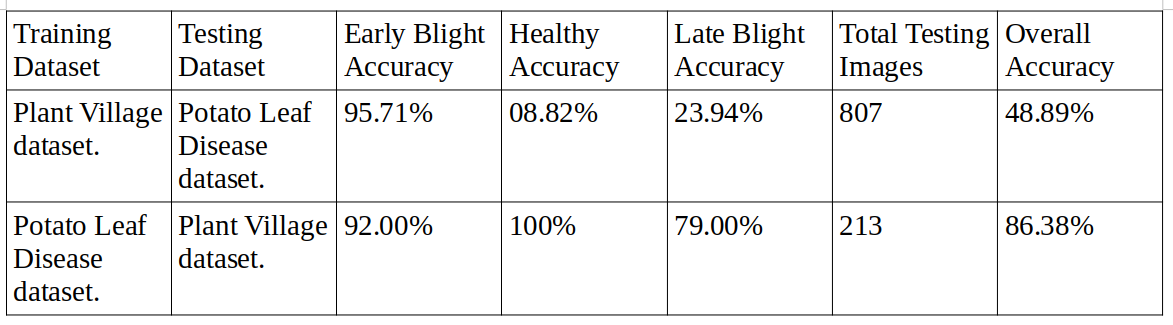
\includegraphics[height=0.15\textheight]  {cross}}
\end{figure}




Our model's cross dataset classification accuracies;\\
\begin{figure}[h]
	\centerline{\small 
		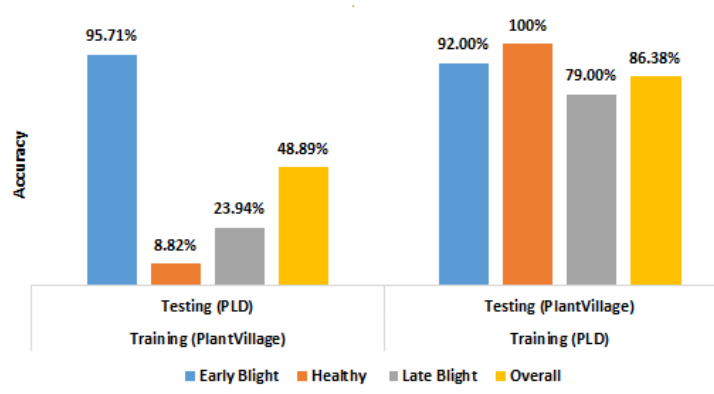
\includegraphics[height=0.25\textheight]  {c1}}
\end{figure}

\section{Conclusion.}
Therefore from the above results,our proposed performed very well on the Potato Leaf Dataset.\\



\newpage
\chapter{Mobile Application Design.}


\section{System Design.}
We used an Architecture diagram,Use case diagram, Data flow diagram and Flow chart.\\

\subsection{Use Case diagram.}
A Use case diagram was used to develop a better understanding of the requirements. This gave us a view of the components and entities of the system under design.\\
The use case identifies the type of interaction and the actor, in particular the farmer, server and administrator of the App, involved.
The use case expounds on the system in detail.\\

\begin{figure}[h]
	\centerline{\small 
		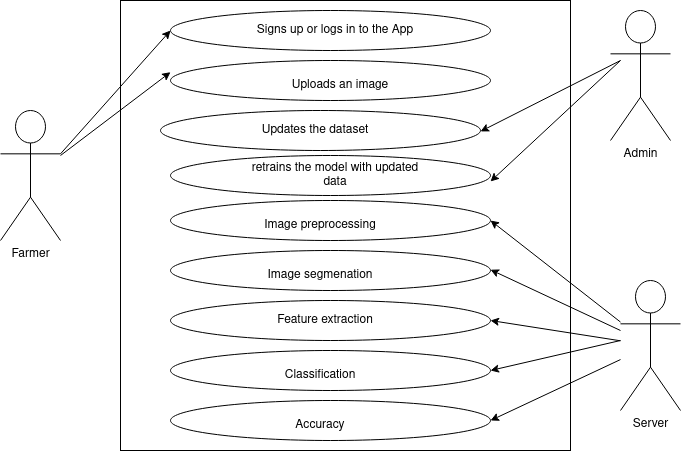
\includegraphics[height=0.3\textheight]  {usecase}}
\end{figure}

\newpage
\subsection{Architecture design.}

\begin{figure}[h]
	\centerline{\small 
		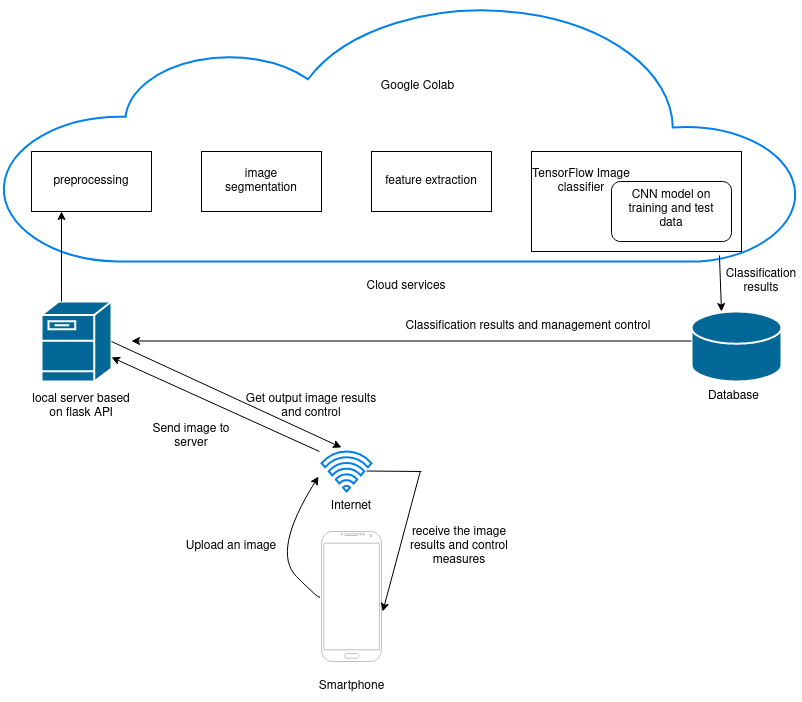
\includegraphics[height=0.5\textheight]  {arch}}
\end{figure}

\subsection{Data flow diagram.}
A data flow diagram was used to represent the system as a set of activities, each of which carries out some data transformation.\\

It showed what kinds of data needed to be input to and output from the system, where the data came from and go to, and where the data was be stored. It also showed how the input to the process was transformed to an output.\\

In level 0 DFD input is an leaf Image then analysis process is
done on that infected leaf the output result is as disease result.\\
\begin{figure}[h]
	\centerline{\small 
		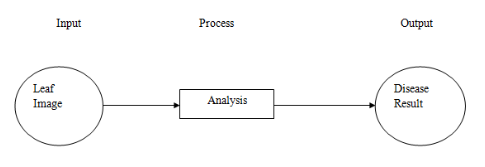
\includegraphics[height=0.15\textheight]  {e}}
\end{figure}

\newpage
In level 1 DFD input is an leaf Image is taken by android
camera or digital camera then analysis process is done by
using some image processing techniques on that infected leaf
then the output result is as disease result produced disease
name ,remedy uses and disease details.\\

\begin{figure}[h]
	\centerline{\small 
		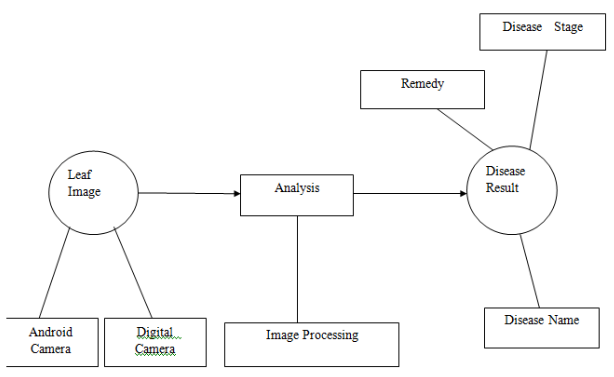
\includegraphics[height=0.3\textheight]  {f}}
\end{figure}

\newpage
\subsection{Flow chart.}
The flow chart represents the dynamic behavior of the objects and classes that have been identified as part of the system.
The flow chart helped us describe the plan in order to perform the different tasks. It showed what was done when the decision was made and when to go to each process as a result. The flow chart helped us build a step by step picture of the processes of our system.\\

\begin{figure}[h]
	\centerline{\small 
		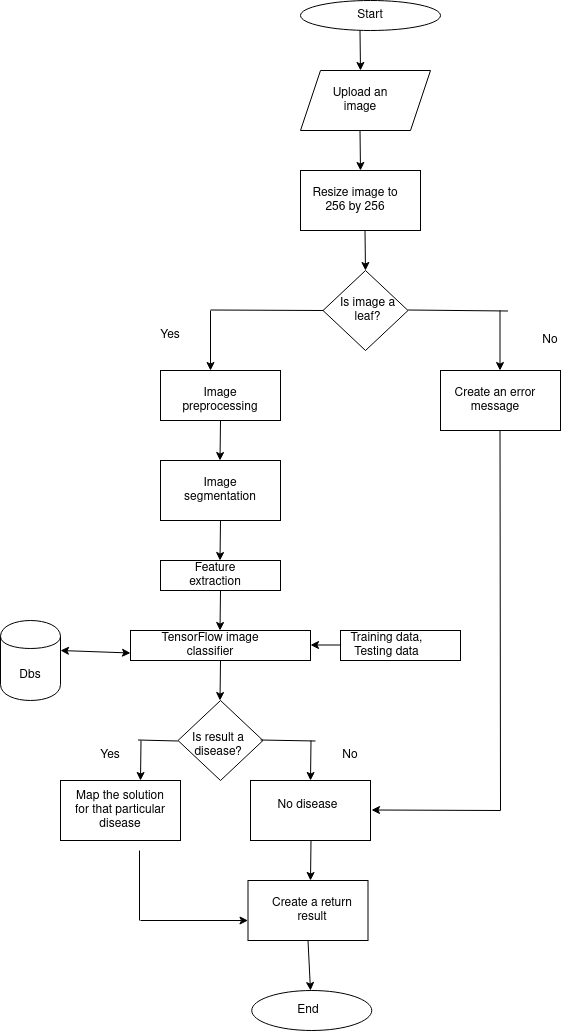
\includegraphics[height=0.5\textheight]  {flowchart}}
\end{figure}

\section{Technology decisions.}

\subsection{Android Application Development.}
The goal for this project was to deliver a proof of concept application so that farmers can leaf images and
gain predictions from a model. To do this, an Android application was developed with an integrated deep
learning model. The Android app was built using the Flutter framework for Dart programming language integrated with the machine learning model built using Python programming language with a Flask framework API.\\

\subsection{Flutter.}
Flutter is an open-source UI software development kit created by Google. It is used to develop cross platform applications for Android, iOS, Linux, Mac, Windows, Google Fuchsia,Web platform, [75] and the web from a single codebase.[76] \\

\subsection{Flask.}
Flask is a micro web framework that uses Python. It is extremely flexible, minimalist and easy to set up.
Flask is also BSD Licensed which allows Flask to be further modified[77]. The great feature about Flask is
that is very flexible and minimalist to use.\\
Flask was used for API.\\




\section{System implementation.}
In the implementation stage, an Android app was developed.\\

\subsection{Android App features.}
The Android application has the following features after it was developed; \\
\begin{itemize}
	\item Authentication using Google OAuth for the case of logging in or signing into the application.\\
	\item User Profile page containing user details like photo and email address.\\
	\item Usage of camera or device media to get an image of the crop.\\
	\item Preview of the image and sending it to API, for disease detection.\\
	\item A result page showing detected plant disease and remedy or solution.\\
	\item Generating a PDF report to save/share the predicted disease details to other users.\\
	\item Option of sending the generated result as a notification warning to other users.\\
	
	
\end{itemize}

\newpage
\subsection{Android App Interfaces.}

Login screen.\\
\begin{figure}[h]
	\centerline{\small 
		
\includegraphics[height=0.25\textheight]  {login}}
\end{figure}

Login with Gmail account for security.\\
\begin{figure}[h]
	\centerline{\small 
		
\includegraphics[height=0.25\textheight]  {home}}
\end{figure}


\newpage
Image Preview.\\
\begin{figure}[h]
	\centerline{\small 
		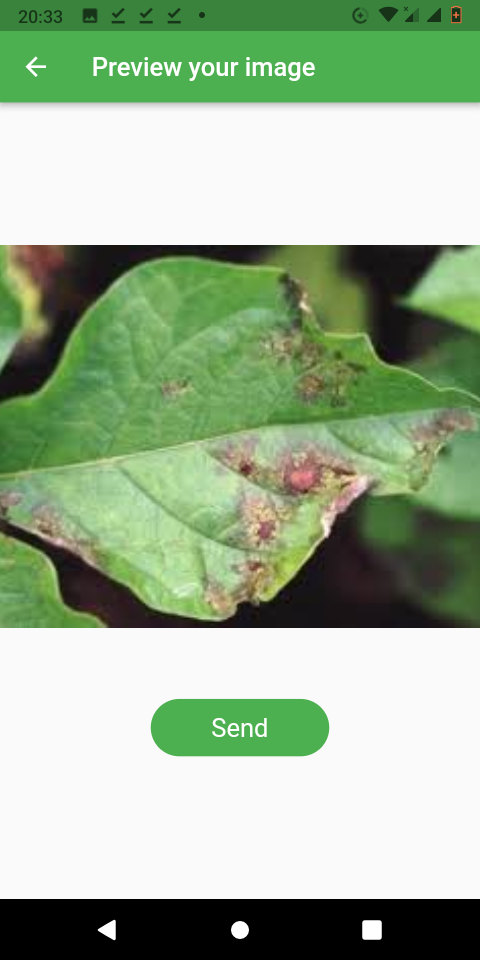
\includegraphics[height=0.20\textheight]  {preview}}
\end{figure}

\begin{figure}[h]
	\centerline{\small 
		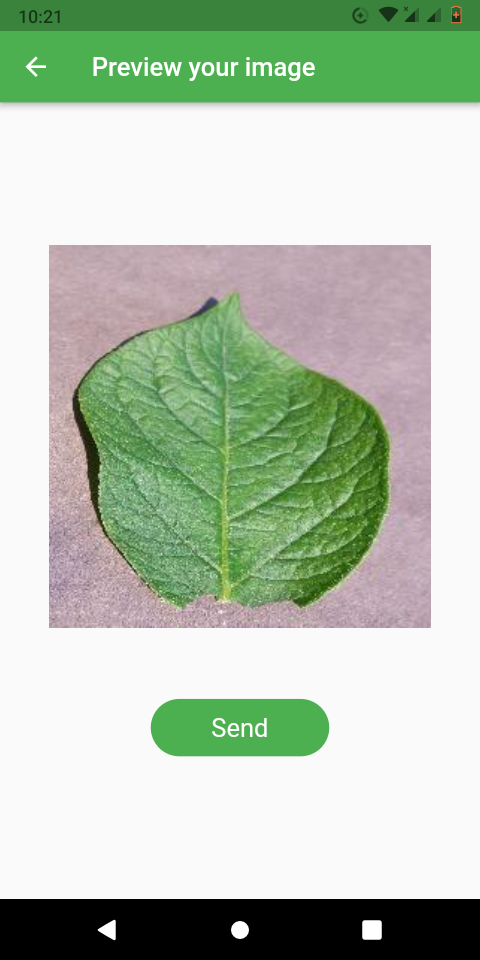
\includegraphics[height=0.20\textheight]  {h1}}
\end{figure}

\begin{figure}[h]
	\centerline{\small 
		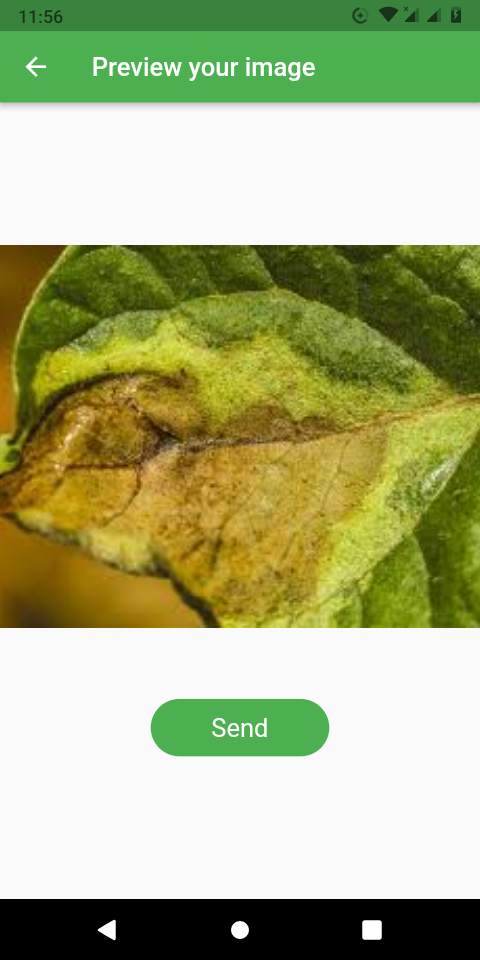
\includegraphics[height=0.20\textheight]  {h3}}
\end{figure}

\newpage
Image results with solutions respectively.\\
\begin{figure}[h]
	\centerline{\small 
		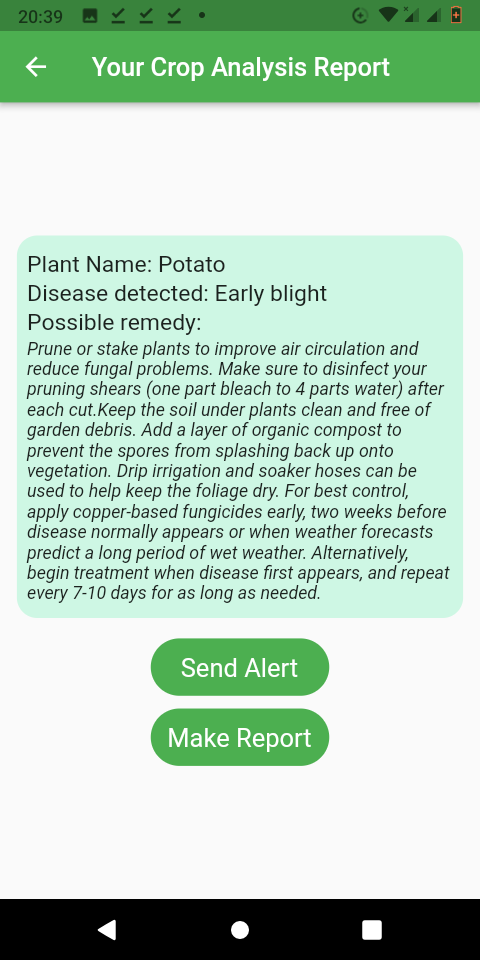
\includegraphics[height=0.25\textheight]  {r2}}
\end{figure}

\begin{figure}[h]
	\centerline{\small 
		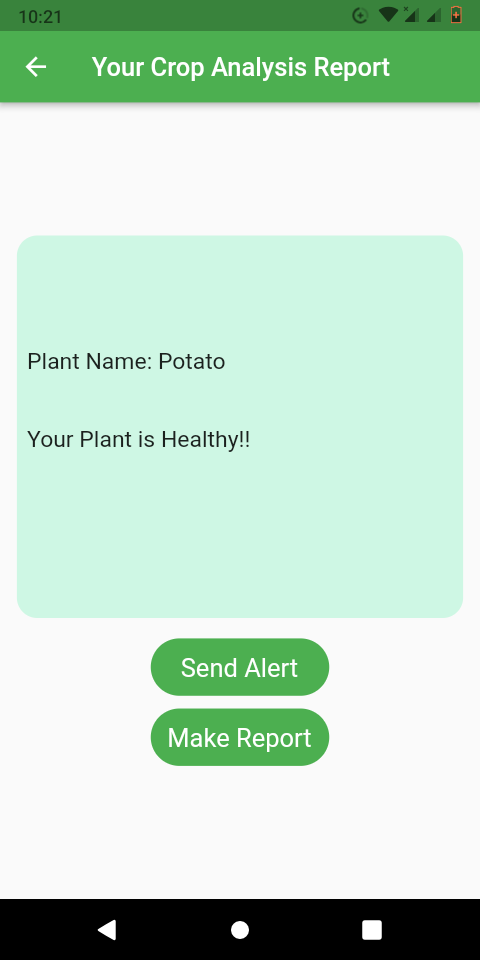
\includegraphics[height=0.20\textheight]  {h2}}
\end{figure}

\begin{figure}[h]
	\centerline{\small 
		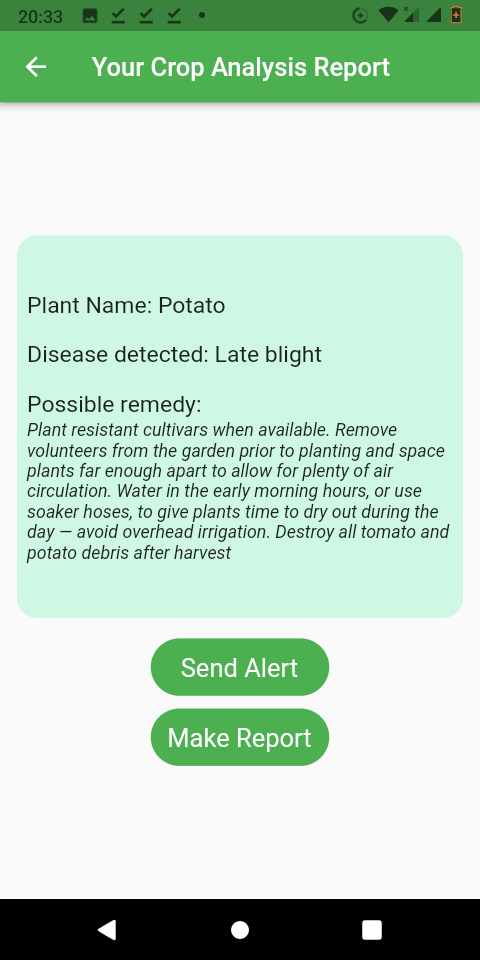
\includegraphics[height=0.25\textheight]  {r1}}
\end{figure}



\newpage
\chapter{Conclusion and Future work.}

\section{Conclusion.}
Deep learning techniques perform significantly in plant leaf disease detection to improve crop productivity and quality by controlling the biotic variables that cause severe crop yield losses.\\

In this research study, a fast and straight forward deep learning model for Irish potato leaf disease recognition was proposed to classify Irish potato leaf diseases. The model at first extracted the Irish potato leaves from plant image using image segmentation technique, a CNN was then developed to classify early blight, lat blight and healthy class from the leaf images. At the same time, it considered the effect of environmental factors on Irish potato leaf images.\\

Experimental studies were also conducted on different datasets with and without data augmentation. Performance of our model was also evaluated on the cross dataset where the model's performance on the Potato Leaf Disease dataset out performed the one on Plant village dataset as it was trained with and without data augmentation thus achieving 99.75\% overall accuracy, high precision, Recall, F1 score and ROC curve.\\ 


\section{Limitations of our study.}
\begin{itemize}
	\item For this research study, we mainly focused on one crop and that was Irish potatoes.\\
	\item Our model only predicts one leaf image at a time ie the background should contain nothing or no other leaf or leaves.\\
	\item For this research study, we only focused on two diseases for the Irish potatoes namely Early blight and Late blight with also the Healthy class too.\\
	\item Our model only predicts a single leaf disease and not multiple leaf diseases for a single leaf.\\
\end{itemize}



\section{Future work.}
In future, this research would be extended to multiple diseases detection on a single leaf
and to localise the diseases, disease severity estimation, develop
IoT-based real-time monitoring system, develop a website and launch a mobile application to predict multiple diseases in many different crops.\\



\newpage
\chapter{Appendix and References.}
\section{References.}
\begin{thebibliography}{100}  % 100 is a random guess of the total number of %references

	\bibitem{1} Sushil R.Kamlapurkar “Detection of Plant Leaf Diseases
	Using Image Processing Approach “International Journal of Scientific and Research 2,February 2016.
	\bibitem{2} MITTAL, S. \& TRIPATHI, G. 2009. Role of Mobile Phone Technology in Improving Small Farm Productivity1. Agricultural Economics Research Review,22,451-459.
	\bibitem{3}  Fletcher, Jacqueline; Stack, James P. "Surveillance Strategies§AGRICULTURAL BIOSECURITY: THREATS AND IMPACTS FOR PLANT PATHOGENS". NCBI Bookshelf (National Center for Biotechnology Information). National Academies Press (National Academy of Sciences). Retrieved 2021-02-12.
	\bibitem{4} Carvajal-Yepes, M.; Cardwell, K.; Nelson, A.; Garrett, K. A.; Giovani, B.; Saunders, D. G. O.; Kamoun, S.; Legg, J. P.; Verdier, V.; Lessel, J.; Neher, R. A.; Day, R.; Pardey, P.; Gullino, M. L.; Records, A. R.; Bextine, B.; Leach, J. E.; Staiger, S.; Tohme, J. (2019-06-27). "A global surveillance system for crop diseases" (PDF). Science. American Association for the Advancement of Science (AAAS). 364 (6447): 1237–1239. 
	\bibitem{5} https://rightstracker.org/en/metric/food
	\bibitem{6} V. Singh and A. K. Misra, “Detection of plant leaf diseases using image segmentation and soft computing techniques,” Information Processing in Agriculture, vol. 4, no. 1, pp. 41–49, 2017. 
	\bibitem{7} S. P. Mohanty, D. P. Hughes, and S. Marcel, “Using deep learning for image-based plant disease detection,” Frontiers in Plant Science, vol. 7, p. 1419, 2016.
	\bibitem{8} Chowdhury, M.E.; Khandakar, A.; Ahmed, S.; Al-Khuzaei, F.; Hamdalla, J.; Haque, F.; Mamun, B.I.R.; Ahmed, A.S.; Nasser, A.E.
	Design, construction and testing of iot based automated indoor vertical hydroponics farming test-bed in Qatar. Sensors 2020, 20,
	5637. [CrossRef] [PubMed]
	\bibitem{9} Strange, R.N.; Scott, P.R. Plant disease: A threat to global food security. Annu. Rev. Phytopathol. 2005, 43, 83–116. [CrossRef]
	\bibitem{10} Oerke, E.-C. Crop losses to pests. J. Agric. Sci. 2006, 144, 31–43. [CrossRef]
	\bibitem{11} Touati, F.; Khandakar, A.; Chowdhury, M.E.; Antonio, S., Jr.; Sorino, C.K.; Benhmed, K. Photo-Voltaic (PV) monitoring system,
	performance analysis and power prediction models in Doha, Qatar. In Renewable Energy; IntechOpen: London, UK, 2020.
	\bibitem{12} Khandakar, A.; Chowdhury, M.E.H.; Kazi, M.K.; Benhmed, K.; Touati, F.; Al-Hitmi, M.; Gonzales, A.S.P., Jr. Machine learning
	based photovoltaics (PV) power prediction using different environmental parameters of Qatar. Energies 2019, 12, 2782. [CrossRef]
	\bibitem{13} Chowdhury, M.H.; Shuzan, M.N.I.; Chowdhury, M.E.; Mahbub, Z.B.; Uddin, M.M.; Khandakar, A.; Mamun, B.I.R. Estimating
	blood pressure from the photoplethysmogram signal and demographic features using machine learning techniques. Sensors 2020,
	20, 3127. [CrossRef]
	\bibitem{14} Chowdhury, M.E.; Khandakar, A.; Alzoubi, K.; Mansoor, S.; Tahir, A.M.; Reaz, M.B.I.; Nasser, A.-E. Real-time smart-digital
	stethoscope system for heart diseases monitoring. Sensors 2019, 19, 2781.
	\bibitem{15} Rahman, T.; Khandakar, A.; Kadir, M.A.; Islam, K.R.; Islam, K.F.; Mazhar, R.; Tahir, R.; Mohammad, T.I.; Saad, B.A.K.; Mohamed,
	A.A.; et al. Reliable tuberculosis detection using chest X-ray with deep learning, segmentation and visualization. IEEE Access
	2020, 8, 191586–191601. [CrossRef]
	\bibitem{16} Tahir, A.; Qiblawey, Y.; Khandakar, A.; Rahman, T.; Khurshid, U.; Musharavati, F.; Islam, M.T.; Kiranyaz, S.; Chowdhury, M.E.H.
	Coronavirus: Comparing COVID-19, SARS and MERS in the eyes of AI. arXiv 2020, arXiv:2005.11524.
	\bibitem{17} Chowdhury, M.E.; Rahman, T.; Khandakar, A.; Mazhar, R.; Kadir, M.A.; Mahbub, Z.B.; Atif, I.; Nasser, A.-E.; Khan, M.S.; Islam,
	K.R. Can AI help in screening viral and COVID-19 pneumonia? IEEE Access 2020, 8, 132665–132676. [CrossRef]
	\bibitem{18} Rahman, T.; Chowdhury, M.E.; Khandakar, A.; Islam, K.R.; Islam, K.F.; Mahbub, Z.B.; Muhammad, A.K.; Saad, K. Transfer
	learning with deep convolutional neural network (CNN) for pneumonia detection using chest X-ray. Appl. Sci. 2020, 10, 3233.
	[CrossRef]
	\bibitem{19} Chowdhury, M.E.; Rahman, T.; Khandakar, A.; Al-Madeed, S.; Zughaier, S.M.; Hassen, H.; Mohammad, T.I. An early warning
	tool for predicting mortality risk of COVID-19 patients using machine learning. arXiv 2020, arXiv:2007.15559.
	\bibitem{20} Chouhan, S.S.; Kaul, A.; Singh, U.P.; Jain, S. Bacterial foraging optimization based radial basis function neural network (BRBFNN)
	for identification and classification of plant leaf diseases: An automatic approach towards plant pathology. IEEE Access 2018, 6,
	8852–8863. [CrossRef]
	\bibitem{21} LeCun, Y.; Haffner, P.; Bottou, L.; Bengio, Y. Object recognition with gradient-based learning. In Shape, Contour and Grouping in
	Computer Vision; Springer: Berlin/Heidelberg, Germany, 1999; pp. 319–345.
	\bibitem{22} LeCun, Y.; Haffner, P.; Bottou, L.; Bengio, Y. Object recognition with gradient-based learning. In Shape, Contour and Grouping in
	Computer Vision; Springer: Berlin/Heidelberg, Germany, 1999; pp. 319–345.
	\bibitem{23} Arya, S.; Singh, R. A Comparative Study of CNN and AlexNet for Detection of Disease in Potato and Mango leaf. In Proceedings
	of the 2019 International Conference on Issues and Challenges in Intelligent Computing Techniques (ICICT), Ghaziabad, India,
	27–28 September 2019; pp. 1–6.
	\bibitem{24} Arya, S.; Singh, R. A Comparative Study of CNN and AlexNet for Detection of Disease in Potato and Mango leaf. In Proceedings
	of the 2019 International Conference on Issues and Challenges in Intelligent Computing Techniques (ICICT), Ghaziabad, India,
	27–28 September 2019; pp. 1–6.
	\bibitem{25} Geetharamani, G.; Pandian, A. Identification of plant leaf diseases using a nine-layer deep convolutional neural network. Comput.
	Electr. Eng. 2019, 76, 323–338.
	\bibitem{26} Kamal, K.; Yin, Z.; Wu, M.; Wu, Z. Depthwise separable convolution architectures for plant disease classification. Comput.
	Electron. Agric. 2019, 165, 104948.
	\bibitem{27} Khamparia, A.; Saini, G.; Gupta, D.; Khanna, A.; Tiwari, S.; de Albuquerque, V.H.C. Seasonal Crops Disease Prediction and
	Classification Using Deep Convolutional Encoder Network. Circuits Syst. Signal Process. 2019, 39, 818–836.
	\bibitem{28} Hughes, D.; Salathé, M. An open access repository of images on plant health to enable the development of mobile disease
	diagnostics. arXiv 2015, arXiv:1511.08060.
	\bibitem{29} Baker, N.T.; Capel, P.D. Environmental Factors that Influence the Location of Crop Agriculture in the Conterminous United States; US
	Department of the Interior, US Geological Survey: Reston, VA, USA, 2011.
	\bibitem{30} Howard, A.G.; Zhu, M.; Chen, B.; Kalenichenko, D.; Wang, W.; Weyand, T.; Andreetto, M.; Adam, H. Mobilenets: Efficient
	convolutional neural networks for mobile vision applications. arXiv 2017, arXiv:1704.04861.
	\bibitem{31} Liang, Q.; Xiang, S.; Hu, Y.; Coppola, G.; Zhang, D.; Sun, W. PD2SE-Net: Computer-assisted plant disease diagnosis and severity
	estimation network. Comput. Electron. Agric. 2019, 157, 518–529
	\bibitem{} Sladojevic S, Arsenovic M, Anderla A, Culibrk D and Stefanovic D (2016)
	Deep neural networks based recognition of plant diseases by leaf image clas-
	sification. Computational Intelligence and Neuroscience 2016, 3289801.
	\bibitem{} Mohanty SP, Hughes DP and Salathé M (2016) Using deep learning for
	image-based plant disease detection. Frontiers in Plant Science 7, 1419.
	doi: 10.3389/fpls.2016.01419.
	\bibitem{} Amara J, Bouaziz B and Algergawy A (2017) A deep learning-based
	approach for banana leaf diseases classification. In Mitschang B (ed.),
	Datenbanksysteme für Business, Technologie und Web (BTW 2017) –
	Workshopband. Lecture Notes in Informatics (LNI). Stuttgart, Germany:
	Gesellschaft für Informatik, pp. 79–88.
	\bibitem{} Chen Y, Lin Z, Zhao X, Wang G and Gu Y (2014) Deep learning-based clas-
	sification of hyperspectral data. IEEE Journal of Selected Topics in Applied
	Earth Observations and Remote Sensing 7, 2094–2107.
	\bibitem{} Luus FP, Salmon BP, van den Bergh F and Maharaj BT (2015) Multiview
	deep learning for land-use classification. IEEE Geoscience and Remote
	Sensing Letters 12, 2448–2452.
	\bibitem{} Lu H, Fu X, Liu C, Li LG, He YX and Li NW (2017) Cultivated land infor-
	mation extraction in UAV imagery based on deep convolutional neural net-
	work and transfer learning. Journal of Mountain Science 14, 731–741.
	\bibitem{} Kussul N, Lavreniuk M, Skakun S and Shelestov A (2017) Deep learning
	classification of land cover and crop types using remote sensing data.
	IEEE Geoscience and Remote Sensing Letters 14, 778–782.
	\bibitem{} Reyes AK, Caicedo JC and Camargo JE (2015) Fine-tuning deep convolu-
	tional networks for plant recognition. In Cappellato L, Ferro N,
	Jones GJF and San Juan E (eds), CLEF2015 Working Notes. Working
	Notes of CLEF 2015 – Conference and Labs of the Evaluation Forum,
	Toulouse, France, September 8–11, 2015. Toulouse: CLEF. Available online
	from: http://ceur-ws.org/Vol-1391/ (Accessed 11 May 2018).
	\bibitem{} Lee SH, Chan CS, Wilkin P and Remagnino P (2015) Deep-plant: plant iden-
	tification with convolutional neural networks. In 2015 IEEE International
	Conference on Image Processing (ICIP). Piscataway, NJ, USA: IEEE,
	pp. 452-456.
	\bibitem{} Grinblat GL, Uzal LC, Larese MG and Granitto PM (2016) Deep learning for
	plant identification using vein morphological patterns. Computers and
	Electronics in Agriculture 127, 418–424.
	\bibitem{42} Hughes, D.; Salathé, M. An open access repository of images on plant health to enable the development of mobile disease
	diagnostics. arXiv 2015, arXiv:1511.08060.
	\bibitem{43} SpMohanty/PlantVillage-Dataset. Available online: https://github.com/spMohanty/PlantVillage-Dataset (accessed on 24
	January 2021).
	\bibitem{44} LeCun Y and Bengio Y (1995) Convolutional networks for images, speech,
	and time series. In Arbib MA (ed.), The Handbook of Brain Theory and
	Neural Networks. Cambridge, MA, USA: MIT Press, pp. 255–258.
	\bibitem{45} Schmidhuber J (2015) Deep learning in neural networks: an overview. Neural
	Networks 61, 85–117.
	\bibitem{46} Pan SJ and Yang Q (2010) A survey on transfer learning. IEEE Transactions
	on Knowledge and Data Engineering 22, 1345–1359.
	\bibitem{47} Canziani A, Paszke A and Culurciello E (2016) An analysis of deep neural
	network models for practical applications. arXiv preprint arXiv:1605.
	07678 [cs.CV].
	\bibitem{48} Schmidhuber J (2015) Deep learning in neural networks: an overview. Neural
	Networks 61, 85–117.
	\bibitem{49} Oquab M, Bottou L, Laptev I and Sivic J (2014) Learning and transferring
	mid-level image representations using convolutional neural networks. In
	Conference on Computer Vision and Pattern Recognition (CVPR).
	Columbus, OH, USA: IEEE, pp. 1717–1724
	\bibitem{50} Abdel-Hamid O, Mohamed AR, Jiang H, Deng L, Penn G and Yu D (2014)
	Convolutional neural networks for speech recognition. IEEE/ACM
	Transactions on Audio, Speech, and Language Processing 22, 1533–1545.
	\bibitem{51} Karpathy A, Toderici G, Shetty S, Leung T, Sukthankar R and Fei-Fei L
	(2014) Large-scale video classification with convolutional neural networks.
	In Proceedings of the Conference on Computer Vision and Pattern
	Recognition (CVPR). Piscataway, NJ, USA: IEEE, pp. 1725–17.
	\bibitem{52} Kim Y (2014) Convolutional neural networks for sentence classification. In
	Proceedings of the 2014 Conference on Empirical Methods in Natural
	Language Processing (EMNLP). Stroudsburg, PA, USA: Association for
	Computational Linguistics, pp. 1746–1751.
	\bibitem{53} Kamilaris A and Prenafeta-Boldú FX (2017) Disaster monitoring using
	unmanned aerial vehicles and deep learning. In Disaster Management for
	Resilience and Public Safety Workshop, Proceedings of EnviroInfo 2017.
	Luxembourg.
	\bibitem{54} Golhani, K.; Balasundram, S.K.; Vadamalai, G.; Pradhan, B. A review of neural networks in plant disease detection using
	hyperspectral data. Inf. Process. Agric. 2018, 5, 354–371.
	\bibitem{55} Aamir, M.; Irfan, M.; Ali, T.; Ali, G.; Shaf, A.; Al-Beshri, A.; Alasbali, T.; Mahnashi, M.H.J.D. An adoptive threshold-based
	multi-level deep convolutional neural network for glaucoma eye disease detection and classification. Diagnostics 2020, 10, 602.
	\bibitem{56} He, K.; Zhang, X.; Ren, S.; Sun, J. Deep residual learning for image recognition. In Proceedings of the IEEE Conference on
	Computer Vision and Pattern Recognition, Las Vegas, NV, USA, 27–30 June 2016; pp. 770–778.
	\bibitem{57} Krizhevsky, A.; Sutskever, I.; Hinton, G. Imagenet classification with deep convolutional networks. In Proceedings of the
	Conference Neural Information Processing Systems (NIPS), Lake Tahoe, NV, USA, 3–6 December 2012; Volume 25, pp. 1097–1105.
	\bibitem{58} Sermanet, P.; Eigen, D.; Zhang, X.; Mathieu, M.; Fergus, R.; LeCun, Y. Overfeat: Integrated recognition, localization and detection
	using convolutional networks. arXiv 2013, arXiv:1312.6229.
	\bibitem{59} Krizhevsky, A. One weird trick for parallelizing convolutional neural networks. arXiv 2014, arXiv:1404.5997.
	\bibitem{60} Simonyan, K.; Zisserman, A. Very deep convolutional networks for large-scale image recognition. arXiv 2014, arXiv:1409.1556.
	\bibitem{61} Szegedy, C.; Liu, W.; Jia, Y.; Sermanet, P.; Reed, S.; Anguelov, D.; Erhan, D.; Vanhoucke, V.; Rabinovich, A. Going deeper with
	convolutions. In Proceedings of the IEEE Conference on Computer Vision and Pattern Recognition, Boston, MA, USA, 7–12 June
	2015; pp. 1–9.
	\bibitem{62} Khalifa, N.E.M.; Taha, M.H.N.; Abou El-Maged, L.M.; Hassanien, A.E. Artificial Intelligence in Potato Leaf Disease Classification:
	A Deep Learning Approach. In Machine Learning and Big Data Analytics Paradigms: Analysis, Applications and Challenges; Springer:
	Berlin/Heidelberg, Germany, 2021; pp. 63–79.
	\bibitem{63} Rozaqi, A.J.; Sunyoto, A. Identification of Disease in Potato Leaves Using Convolutional Neural Network (CNN) Algorithm. In
	Proceedings of the 2020 3rd International Conference on Information and Communications Technology (ICOIACT), Yogyakarta,
	Indonesia, 24–25 November 2020; pp. 72–76.
	\bibitem{64} Sanjeev, K.; Gupta, N.K.; Jeberson, W.; Paswan, S. Early Prediction of Potato Leaf Diseases Using ANN Classifier. Orient. J.
	Comput. Sci. Technol. 2020, 13, 2–4.
	\bibitem{65} Barman, U.; Sahu, D.; Barman, G.G.; Das, J. Comparative Assessment of Deep Learning to Detect the Leaf Diseases of Potato
	based on Data Augmentation. In Proceedings of the 2020 International Conference on Computational Performance Evaluation
	(ComPE), Shillong, India, 2–4 July 2020; pp. 682–687.
	\bibitem{66} Tiwari, D.; Ashish, M.; Gangwar, N.; Sharma, A.; Patel, S.; Bhardwaj, S. Potato leaf diseases detection using deep learning. In
	Proceedings of the 2020 4th International Conference on Intelligent Computing and Control Systems (ICICCS), Madurai, India,
	13–15 May 2020; pp. 461–466.
	\bibitem{67} Lee, T.Y.; Yu, J.Y.; Chang, Y.C.; Yang, J.M. Health Detection for Potato Leaf with Convolutional Neural Network. In Proceedings
	of the 2020 Indo–Taiwan 2nd International Conference on Computing, Analytics and Networks (Indo-Taiwan ICAN), Rajpura,
	India, 7–15 February 2020; pp. 289–293.
	\bibitem{68} Islam, M.; Dinh, A.; Wahid, K.; Bhowmik, P. Detection of potato diseases using image segmentation and multiclass support
	vector machine. In Proceedings of the 2017 IEEE 30th canadian conference on electrical and computer engineering (CCECE),
	Windsor, ON, Canada, 30 April–3 May 2017; pp. 1–4.
	\bibitem{69} Hughes, D.; Salathé, M. An open access repository of images on plant health to enable the development of mobile disease
	diagnostics. arXiv 2015, arXiv:1511.08060.
	\bibitem{70} Welcome to Python.org, . URL https://www.python.org/.
	\bibitem{71} TensorFlow, . URL https://www.tensorflow.org/.
	\bibitem{72} F. Chollet. Keras as a simplified interface to TensorFlow: tutorial. URL https://blog.keras.io/
	keras-as-a-simplified-interface-to-tensorflow-tutorial.html.
	\bibitem{73} Project Jupyter, . URL http://www.jupyter.org.
	\bibitem{74} www.googlecolab.com
	\bibitem{75} https://arstechnica.com/gadgets/2017/05/googles-fuchsia-smartphone-os-dumps-linux-has-a-wild-new-ui/
	\bibitem{76}  Amadeo, Ron (2018-02-27). "Google starts a push for cross-platform app development with Flutter SDK". Ars Technica. Retrieved 2021-06-11.
	\bibitem{77} Welcome | Flask (A Python Microframework), . URL http://flask.pocoo.org/.
	\bibitem{78} "Convolutional Neural Networks (Lenet) — Deeplearning 0.1 Documentation". Deeplearning.net. N.p.,
	2017. Web. 8 Apr. 2017.
	\bibitem{79} "CS231n Convolutional Neural Networks for VisualRecognition", Cs231n.github.io, 2017. [Online].
	Available: http://cs231n.github.io/convolutional-networks/. [Accessed: 08- Apr- 2017].
	\bibitem{80} A.Deshpande,"A Beginner's Guide To Understanding Convolutional Networks", Adeshpande3.github.io, Neural 2017.
	[Online].Available:https://adeshpande3.github.io/adeshpande3.github.io/A-Beginner's-Guide-To-Understanding-Convolutional-Neural-Networks/. [Accessed: 08- Apr- 2017].
	\bibitem{81} Ren, Hansheng; Xu, Bixiong; Wang, Yujing; Yi, Chao; Huang, Congrui; Kou, Xiaoyu; Xing, Tony; Yang, Mao; Tong, Jie; Zhang, Qi (2019). "Time-Series Anomaly Detection Service at Microsoft | Proceedings of the 25th ACM SIGKDD International Conference on Knowledge Discovery \& Data Mining". arXiv:1906.03821. doi:10.1145/3292500.3330680. S2CID 182952311.
	\bibitem{82} Wallach, Izhar; Dzamba, Michael; Heifets, Abraham (2015-10-09). "AtomNet: A Deep Convolutional Neural Network for Bioactivity Prediction in Structure-based Drug Discovery". arXiv:1510.02855 [cs.LG].
	\bibitem{83} Baccouche, Moez; Mamalet, Franck; Wolf, Christian; Garcia, Christophe; Baskurt, Atilla (2011-11-16). "Sequential Deep Learning for Human Action Recognition". In Salah, Albert Ali; Lepri, Bruno (eds.). Human Behavior Unterstanding. Lecture Notes in Computer Science. 7065. Springer Berlin Heidelberg. pp. 29–39. CiteSeerX 10.1.1.385.4740. doi:10.1007/978-3-642-25446-8\_4. ISBN 978-3-642-25445-1.
	\bibitem{84} Ji, Shuiwang; Xu, Wei; Yang, Ming; Yu, Kai (2013-01-01). "3D Convolutional Neural Networks for Human Action Recognition". IEEE Transactions on Pattern Analysis and Machine Intelligence. 35 (1): 221–231. CiteSeerX 10.1.1.169.4046. doi:10.1109/TPAMI.2012.59. ISSN 0162-8828. PMID 22392705. S2CID 1923924.
	\bibitem{85} Bai, Shaojie; Kolter, J. Zico; Koltun, Vladlen (2018-04-19). "An Empirical Evaluation of Generic Convolutional and Recurrent Networks for Sequence Modeling". arXiv:1803.01271 [cs.LG].
	\bibitem{86} Tsantekidis, Avraam; Passalis, Nikolaos; Tefas, Anastasios; Kanniainen, Juho; Gabbouj, Moncef; Iosifidis, Alexandros (July 2017). "Forecasting Stock Prices from the Limit Order Book Using Convolutional Neural Networks". 2017 IEEE 19th Conference on Business Informatics (CBI). Thessaloniki, Greece: IEEE: 7–12. doi:10.1109/CBI.2017.23. ISBN 978-1-5386-3035-8. S2CID 4950757.
	\bibitem{87} Yu, Fisher; Koltun, Vladlen (2016-04-30). "Multi-Scale Context Aggregation by Dilated Convolutions". arXiv:1511.07122 [cs.CV]
	\bibitem{88} Borovykh, Anastasia; Bohte, Sander; Oosterlee, Cornelis W. (2018-09-17). "Conditional Time Series Forecasting with Convolutional Neural Networks". arXiv:1703.04691 [stat.ML]
	\bibitem{89} Mittelman, Roni (2015-08-03). "Time-series modeling with undecimated fully convolutional neural networks". arXiv:1508.00317 [stat.ML].
	\bibitem{90} Chen, Yitian; Kang, Yanfei; Chen, Yixiong; Wang, Zizhuo (2019-06-11). "Probabilistic Forecasting with Temporal Convolutional Neural Network". arXiv:1906.04397 [stat.ML].
	\bibitem{91} Grefenstette, Edward; Blunsom, Phil; de Freitas, Nando; Hermann, Karl Moritz (2014-04-29). "A Deep Architecture for Semantic Parsing". arXiv:1404.7296 [cs.CL].
	\bibitem{92} Mesnil, Gregoire; Deng, Li; Gao, Jianfeng; He, Xiaodong; Shen, Yelong (April 2014). "Learning Semantic Representations Using Convolutional Neural Networks for Web Search – Microsoft Research". Microsoft Research. Retrieved 2015-12-17.
	\bibitem{93} Kalchbrenner, Nal; Grefenstette, Edward; Blunsom, Phil (2014-04-08). "A Convolutional Neural Network for Modelling Sentences". arXiv:1404.2188 [cs.CL].
	\bibitem{94} Kim, Yoon (2014-08-25). "Convolutional Neural Networks for Sentence Classification". arXiv:1408.5882 [cs.CL].
	\bibitem{95} Collobert, Ronan, and Jason Weston. "A unified architecture for natural language processing: Deep neural networks with multitask learning."Proceedings of the 25th international conference on Machine learning. ACM, 2008.
	\bibitem{96} Collobert, Ronan; Weston, Jason; Bottou, Leon; Karlen, Michael; Kavukcuoglu, Koray; Kuksa, Pavel (2011-03-02). "Natural Language Processing (almost) from Scratch". arXiv:1103.0398 [cs.LG].
	\bibitem{97} Tim Pyrkov; Konstantin Slipensky; Mikhail Barg; Alexey Kondrashin; Boris Zhurov; Alexander Zenin; Mikhail Pyatnitskiy; Leonid Menshikov; Sergei Markov; Peter O. Fedichev (2018). "Extracting biological age from biomedical data via deep learning: too much of a good thing?". Scientific Reports. 8 (1): 5210. Bibcode:2018NatSR...8.5210P. doi:10.1038/s41598-018-23534-9. PMC 5980076. PMID 29581467.
	
\end{thebibliography}

\newpage
\section{Github repository link.}
https://github.com/Group4Day2019/CS21-2-Group\_2/tree/main\\

\section{Places to visit.}
Visits were done to Irish potato gardens of some of the nearby farmers.\\
More data inform of images in JPG format were collected from the College of Agriculture, Makerere University.\\ 

\vspace{5mm}


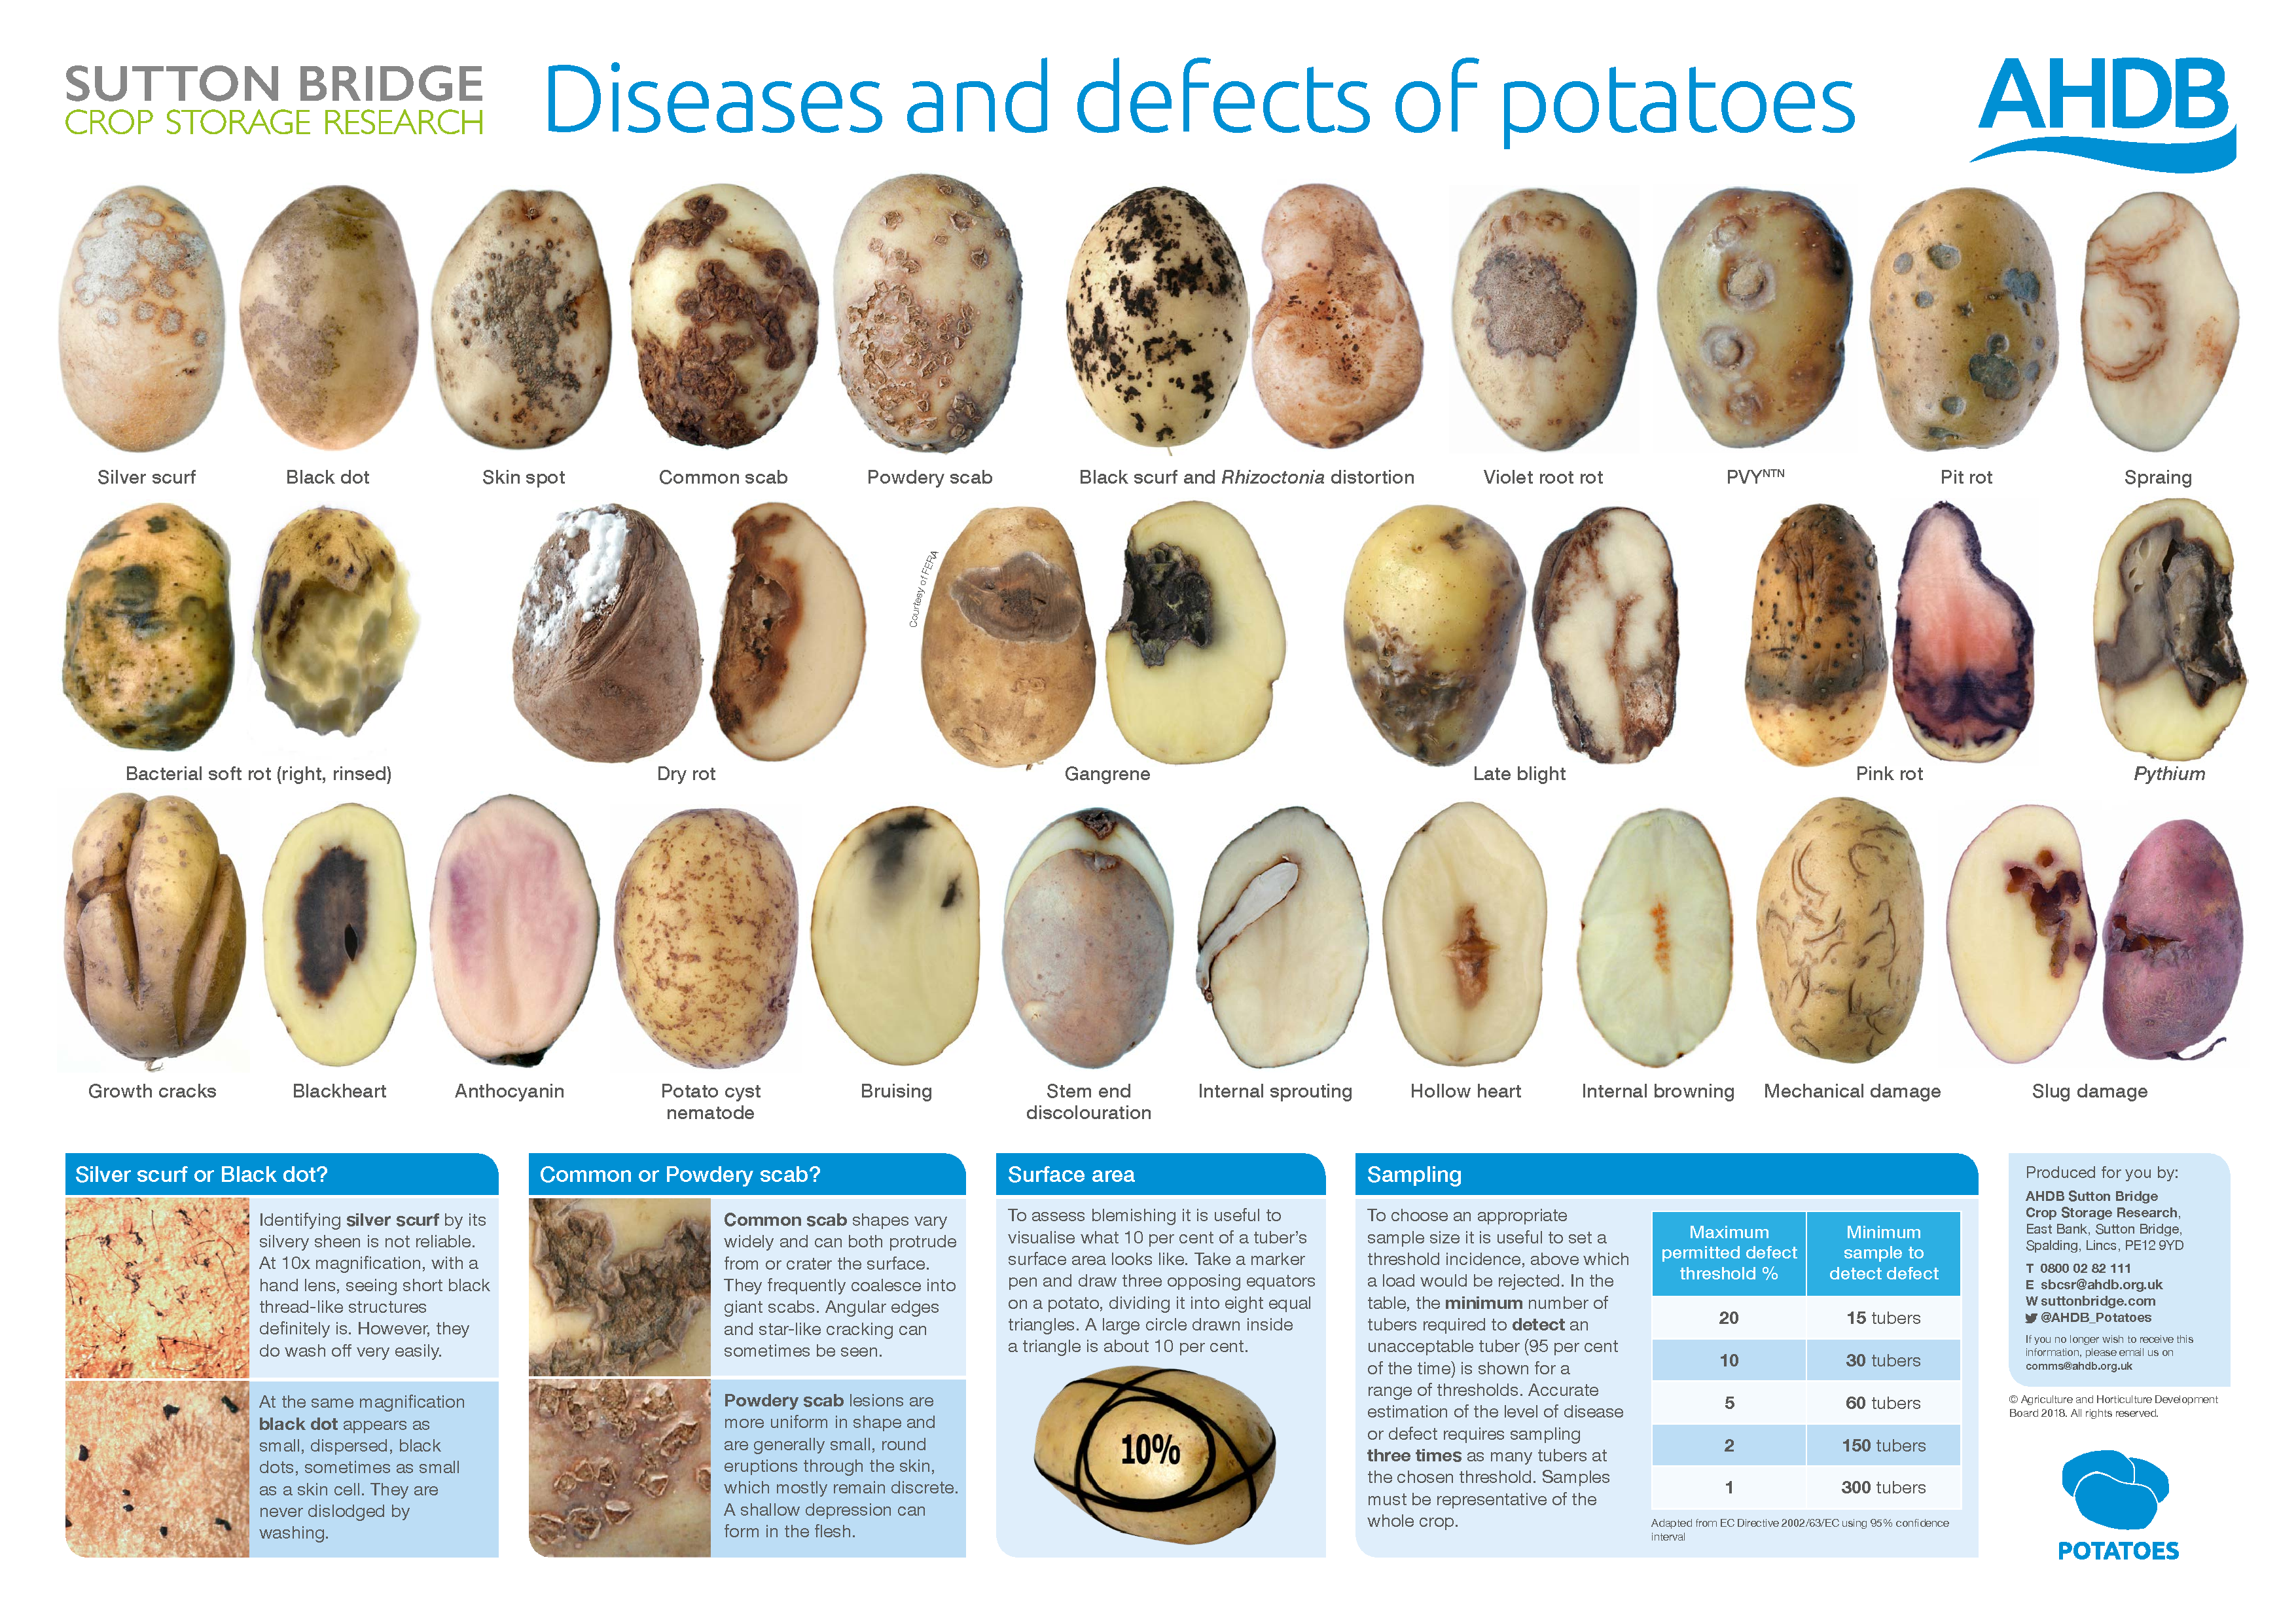
\includepdf[pages=1-1, pagecommand={\thispagestyle{plain}},
addtotoc={1, section, 1, Diseases and defects of potatoes., app:liposyn}
]{ian} 



\end{document}